\section{INVESTIGACIÓN DE MERCADO}

\subsection{Investigación y revisión sobre aplicaciones y tecnologías similares}

Se investigan aplicaciones con funcionalidades parecidas a la solución propuesta por Señas Chapinas. 

\subsubsection{Hand Talk Translator}

Es una aplicación gratuita para dispositivos Android e iOS diseñada para mejorar la comunicación entre la comunidad sorda y las personas que pueden oír. Esta traduce texto, ya sea en texto o en audio, al lenguaje de señas americanas. Esto se realiza por medio de Hugo, un avatar tridimensional animado por IA, que facilita la traducción y el aprendizaje. Los usuarios tienen la opción de repetir las traducciones, modificar la velocidad de Hugo, guardar y calificar sus traducciones preferidas. También pueden crear mensajes en GIF para compartir y personalizar la apariencia de Hugo en su tienda \cite{Foggetti2023}.

    
\begin{itemize}
    \item \textbf{Funcionalidades destacadas}
    \begin{itemize}
        \item Traducción de frases a lengua de señas ASL mostrado a través de animación 3D.
        \item Opción de compartir por GIF en redes sociales.
        \item Opción de guardar traducción en favoritos.
        \item Opción de repetir la traducción y cambiar la velocidad de reproducción.
    \end{itemize}
    
    \item \textbf{Características de Diseño}
    \begin{itemize}
        \item Incorpora elementos interactivos y de personalización para mejorar la experiencia del usuario. Esto vuelve la aplicación más atractiva y personal.
        \item Animación fluida de Hugo, que facilita el seguimiento visual de las señas.
        \item Interfaz intuitiva y simple que permite una navegación sencilla por las distintas funciones de la aplicación.
        \item Uso de color naranja que induce calidez, alegría, optimismo y confianza.
        \item Los íconos y botones son grandes y están claramente etiquetados, lo cual es útil para una rápida identificación de la funcionalidad.
        \item La interfaz es responsiva.
    \end{itemize}

    \item \textbf{Comentarios de usuarios}
    \begin{itemize}
        \item Los usuarios solicitan que la aplicación traduzca palabras y no letra por letra.
        \item Los usuarios solicitan mayor cantidad de palabras disponibles para traducción a señas.
    \end{itemize}
\end{itemize}

\begin{figure} [h]
    \centering
    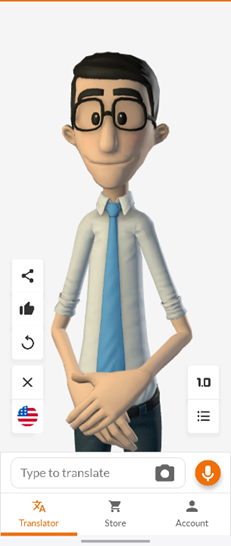
\includegraphics[width=0.25\linewidth]{figuras/handTalk.png}
    \caption{Muestra de aplicación “Hand Talk Translator”}
    \label{fig:enter-label}
\end{figure}


\subsubsection{SLAIT – Real-time Sign Language Translator with AI}

Es una aplicación en fase beta que ofrece servicios de traducción de lengua de señas americanas en tiempo real para dispositivos móviles, web, entre otros. Utiliza inteligencia artificial para realizar traducciones en tiempo real, otorgando facilidad de comunicación para comunicación diaria, salud, educación y oficina. Esta aplicación tendrá modalidad de pago, aunque permite ser parte de la aplicación beta sin costo pero con previo análisis del caso por la empresa \cite{SLAIT}.

\begin{itemize}
    \item \textbf{Funcionalidades destacadas}
    \begin{itemize}
        \item Traducción instantánea de voz a texto.
        \item Traducción instantánea de señas a texto.
    \end{itemize}

    \item \textbf{Características de Diseño}
    \begin{itemize}
        \item Diseño simple y amigable con el usuario.
    \end{itemize}
\end{itemize}

\subsubsection{Lenguaje de Señas IA}

La aplicación ofrece una plataforma de traducción de señas ASL a texto y viceversa, con múltiples funciones como búsqueda por categoría, emoji y alfabeto, y soporte para diez idiomas. Con más de 2,600 señas reconocidas, busca facilitar la comunicación y el aprendizaje del lenguaje de señas \cite{LenguajeDeSeñasIA}.

\begin{itemize}
    \item \textbf{Funcionalidades destacadas}
    \begin{itemize}
        \item Grabación de señas ASL para su reconocimiento y traducción a 10 diferentes idiomas.
        \item Traducción de frases en inglés a señas ASL, seña por seña.
        \item Búsqueda de señas por emoji, categoría, palabra y alfabéticamente.
    \end{itemize}

    \item \textbf{Características de Diseño}
    \begin{itemize}
        \item Paleta de colores e iconografía básica.
        \item Diseño confuso y apretado.
    \end{itemize}
\end{itemize}

\begin{figure} [h]
    \centering
    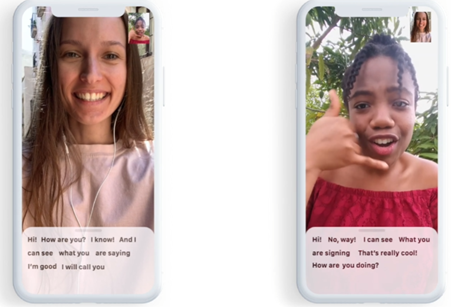
\includegraphics[width=0.5\linewidth]{figuras/slait.png}
    \caption{Muestra de aplicación “SLAIT”}
    \label{fig:enter-label}
\end{figure}

\subsubsection{AI Sign: Sign Language}

Es una aplicación para IOS que utiliza inteligencia artificial para reconocer más de 100 señas americanas. Tiene dos modos: reconocimiento de acciones en tiempo real y captura de datos para mejorar la precisión del modelo de aprendizaje automático \cite{AISign2023}.

\begin{itemize}
    \item \textbf{Funcionalidades destacadas}
    \begin{itemize}
        \item Capacidad de reconocimiento en tiempo real.
        \item Contiene un modo de ayuda y ajustes de configuración para personalizar la experiencia.
    \end{itemize}

    \item \textbf{Características de diseño}
    \begin{itemize}
        \item Muestra de toma de datos de las señas, señalando puntos clave de la mano.
        \item No hay paleta de colores, se usan elementos gráficos básicos.
        \item Botones poco amigables y descriptivos.
    \end{itemize}
\end{itemize}

\begin{figure}[h]
    \centering
    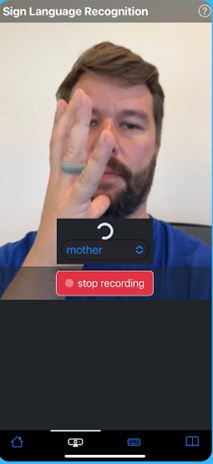
\includegraphics[width=0.25\linewidth]{figuras/applenguasenasia.png}
    \caption{Muestra de aplicación “Lenguaje de señas IA”}
    \label{fig:enter-label}
\end{figure}


\subsubsection{Sign Language Translator AI}

Es una aplicación móvil diseñada para reconocer y traducir el lenguaje de señas coreano. Utiliza inteligencia artificial para interpretar señas en tiempo real, buscando facilitar la comunicación para las personas sordomudas. La aplicación también fomenta la participación de los usuarios para mejorar su base de datos y aumentar la precisión del reconocimiento de gestos \cite{SignLanguageTranslatorAI}.

\begin{itemize}
    \item \textbf{Funcionalidades destacadas}
    \begin{itemize}
        \item Guías visuales para el posicionamiento correcto ante la cámara, esenciales para el reconocimiento de gestos.
        \item Capacidad de reconocimiento en tiempo real.
        \item Invitación a los usuarios para contribuir con sus propios gestos, ayudando a mejorar la base de datos.
        \item Lista de palabras reconocibles que sigue expandiéndose con las contribuciones de los usuarios.
    \end{itemize}

    \item \textbf{Características de diseño}
    \begin{itemize}
        \item Botones descriptivos.
        \item Interfaz simple y clara.
        \item Diseño intuitivo.
    \end{itemize}
\end{itemize}

\begin{figure} [H]
    \centering
    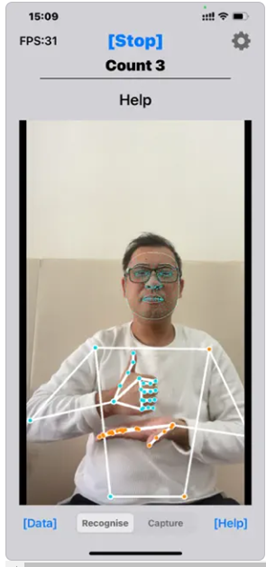
\includegraphics[width=0.25\linewidth]{figuras/ai_sign.png}
    \caption{Muestra de aplicación “AI Sign: Sign Language”}
    \label{fig:enter-label}
\end{figure}

\subsubsection{Resumen de Funcionalidades y Características Destacadas de Aplicaciones Investigadas}

Luego de la investigación previa, se destacan las siguientes funcionalidades:
\begin{itemize}
    \item Espacio para grabar un video con indicadores de posición y luz adecuados para garantizar una captura óptima del vídeo.
    \item Modo ayuda para tutorial.
    \item Botón de compartir para difundir textos traducidos en redes sociales.
    \item Botón de agregar a favoritos la traducción realizada.
    \item Botón de reproducción de voz.
    \item Botón para calificar la traducción.
    \item Historial de videos grabados.
    \item Lista de palabras reconocibles.
\end{itemize}

Asimismo, destacan las siguientes características de diseño:
\begin{itemize}
    \item Diseño limpio e intuitivo.
    \item Paleta de colores atractiva.
    \item Botones descriptivos para mayor comprensión de su función.
\end{itemize}

% ---------------------------------------------------------------------------------------------------------------

\subsection{Investigación de la situación actual de los sordos en Guatemala}

En Guatemala, se estima que hay aproximadamente 240,000 personas sordas, lo que representa el 3\% de la población mayor de cuatro años, según datos del Instituto Nacional de Estadística (INE). Las causas de la sordera son diversas e incluyen factores genéticos, complicaciones durante el nacimiento y enfermedades infecciosas. Uno de los principales desafíos que enfrentan las personas sordas en el país es la comunicación, lo cual limita su capacidad para participar de manera equitativa en la sociedad \cite{CongresoGuatemala} \cite{GobiernoGuatemala2022}.

La lengua de señas reconocida es LENSEGUA. Las personas sordas están dispersas por todo el territorio nacional, pero se estima que la mayoría que saben LENSEGUA están concentradas principalmente en la ciudad capital. En áreas rurales con acceso limitado a la educación, como el norte de Petén, las personas sordas a menudo desarrollan sus propios sistemas de señas \cite{JoshuaProject}. 

El ámbito educativo presenta desafíos notables. A pesar de la existencia de organizaciones como la Asociación Nacional de Sordos de Guatemala, que brinda educación y otros servicios, las oportunidades educativas son escasas, especialmente en áreas rurales. Muchos estudiantes sordos deben alejarse de sus familias para acceder a opciones educativas que incluyan instrucción en lengua de señas. Un gran número de ellos ni siquiera tiene la oportunidad de acceder a una educación básica debido a la escasez de maestros capacitados en lengua de señas. Menos del 50\% recibe educación formal y las escuelas rara vez ofrecen niveles de educación secundaria. Aquellos que persiguen estudios superiores a menudo lo hacen sin la ayuda de intérpretes, lo que complica su aprendizaje y progreso académico. Esto perpetúa un ciclo de desventajas educativas y económicas, con altas tasas de desempleo y dependencia económica entre la comunidad sorda \cite{EndangeredLanguages}.

El desempleo es elevado en esta comunidad debido a las barreras comunicativas y la falta de adaptaciones adecuadas en los lugares de trabajo. La mayoría de las personas sordas vive con sus padres y están relegadas a trabajos de mano de obra básica debido a las barreras para obtener empleos mejor remunerados \cite{EndangeredLanguages}.

A pesar de estos retos, ha habido iniciativas para mejorar la inclusión de las personas sordas en Guatemala. Por ejemplo, el Benemérito Comité Pro-Ciegos y Sordos de Guatemala, en colaboración con SEGEPLAN, ha trabajado en promover la educación inclusiva y el empleo equitativo, aunque la implementación efectiva de estas políticas aún enfrenta obstáculos significativos \cite{GobiernoGuatemala2022}.

%------------------------------------------------------------------------------------------------------

\subsection{Preparación y realización de entrevistas y encuestas}

\subsubsection{Entrevista a Doctor Gonzalez}

El Dr. Gonzalez, médico general con más de 15 años de experiencia, compartió sus reflexiones sobre la importancia de mejorar la comunicación con pacientes sordos. Durante la entrevista, destacó las dificultades que enfrenta en su práctica diaria, particularmente en la correcta comprensión de los síntomas y necesidades de los pacientes sordos, lo cual es fundamental para proporcionar un diagnóstico preciso y un tratamiento efectivo.

El Dr. Gonzalez expresó su entusiasmo por la iniciativa de la aplicación "Señas Chapinas", mencionando que una herramienta de este tipo podría ser revolucionaria para la práctica médica. Resaltó la potencialidad de la app para facilitar una comunicación fluida y precisa con pacientes sordos, reduciendo los malentendidos y aumentando la calidad del cuidado médico. 

\subsubsection{Entrevista a abogada Claudia Barrillas}

En esta entrevista, se abordó el contexto legal de las personas sordomudas en Guatemala, destacando la importancia de proteger sus derechos en los procedimientos judiciales. Se resaltó la necesidad de contar siempre con un intérprete de lengua de señas durante las declaraciones para asegurar una comunicación efectiva. La escasez de intérpretes, sin embargo, puede provocar demoras en los procesos legales. La Licenciada Barrillas enfatizó el valor de una aplicación de traducción de lengua de señas que podría permitir una comunicación más fluida y directa, reduciendo la dependencia de intermediarios y mejorando el acceso a la justicia para las personas sordomudas, fomentando la inclusión y la igualdad.

Se mencionaron casos donde la ausencia de intérpretes resultó en injusticias o malentendidos legales, subrayando la importancia de una comunicación clara y efectiva en el ámbito judicial. Barrillas propuso que una aplicación de traducción de lengua de señas no solo facilitaría la comunicación en procesos legales, sino que también promovería una mayor autonomía para las personas sordomudas, eliminando muchas barreras que enfrentan cotidianamente.

\subsubsection{Entrevista con experta en Lensegua Carmen Lucía}

En esta entrevista se abordaron temas clave sobre la estructura y adaptación del español signado en la lengua de señas. 

Carmen explicó que las personas que nacen sordas generalmente aprenden la lengua de señas como su primer idioma, lo cual posee una gramática y estructura propias, distintas del español hablado. Por otro lado, aquellas que pierden la audición más tarde en la vida pueden intentar adaptar su forma de hablar al español, conservando características del lenguaje oral. Este contraste muestra cómo la forma de comunicación varía significativamente entre quienes han sido sordos desde el nacimiento y quienes se han vuelto sordos posteriormente.

Uno de los desafíos discutidos fue la falta de un estándar unificado en la lengua de señas en Guatemala, lo que lleva al uso de señas específicas en regiones como Quetzaltenango. Esta variabilidad regional complica la comunicación y la educación en lengua de señas. Además, Carmen subrayó la importancia de contar con intérpretes y educadores certificados por el Ministerio de Educación para asegurar utilizar el Lensegua “oficial”. 

También se mencionó que muchas de las señas utilizadas en Guatemala son adaptaciones de la lengua francesa, compartiendo similitudes gramaticales con este idioma. Carmen recomendó la necesidad de investigar más sobre estas reglas gramaticales y consultar documentación específica que pueda profundizar el entendimiento y la correcta aplicación de la lengua de señas.

La discusión también resaltó la relevancia de la posición y el movimiento de las manos en la comunicación a través de señas, dado que pequeñas variaciones pueden alterar significativamente el significado de las palabras. Por ejemplo, las señas para ``hola'' y ``gracias'' son muy parecidas y pueden confundirse fácilmente. 

Finalmente, se recalcó que no siempre es posible traducir todas las palabras directamente a señas, lo que destaca la complejidad de desarrollar recursos efectivos para la comunicación en lengua de señas y la importancia de adaptar continuamente las herramientas educativas y de comunicación para satisfacer las necesidades de la comunidad sorda.


\subsubsection{Entrevista a intérprete en En-Señas Melany Cordero}

Melany Cordero, quien ejerce como intérprete y maestra de nivel medio en En-Señas, acompaña a profesoras en la impartición de clases y asiste en la resolución de dudas de los alumnos. Comenzó su formación en LENSEGUA en la academia y obtuvo su diploma que la acredita como intérprete.

Durante la entrevista, Melany expresó que la propuesta de la aplicación ``Señas Chapinas'' le pareció tanto útil como innovadora. Sugirió la inclusión de elementos como juegos o retos diarios, para fomentar un aprendizaje continuo y efectivo de LENSEGUA entre los usuarios. Propuso, por ejemplo, implementar un juego de memoria o un ejercicio similar a los utilizados en exámenes, donde se presenta una palabra y los usuarios deben seleccionar la seña correcta asociada. Estas actividades no solo mantendrían el interés de los usuarios, sino que también potenciarían su capacidad de aprendizaje y retención de la lengua de señas de manera divertida y desafiante.


\subsubsection{Entrevista a director general de En-Señas Antonio Barrientos}

Antonio desarrolló un interés por la lengua de señas inspirado por su madre, quien también la aprendió y frecuentaba a la comunidad sorda. Motivado por su deseo de entender las conversaciones de este grupo, Antonio se sumergió en el estudio de la lengua de señas y actualmente es intérprete de nivel avanzado y director general de la institución ``En-Señas''.

Durante la entrevista, Antonio señaló que una de las principales complicaciones con la aplicación "Señas Chapinas" es la falta de un estándar uniforme para LENSEGUA. Explicó que existen variaciones significativas en el uso de señas entre los diferentes departamentos de Guatemala, e incluso entre distintas instituciones educativas, lo que puede complicar la precisión de las traducciones. Esta diversidad se debe a la ausencia de una entidad reguladora que estandarice las señas y certifique quiénes están calificados para enseñar LENSEGUA. No obstante, actualmente hay esfuerzos para lograr esta estandarización.

Antonio también destacó la escasez de materiales e información en línea sobre LENSEGUA, así como las deficiencias legislativas que, aunque reconocen la lengua de señas, no establecen un marco regulatorio suficiente para su enseñanza y promoción.

En cuanto a la comunidad sorda, mencionó que existen cuatro categorías distintas: personas que utilizan señas caseras y no interactúan con LENSEGUA, aquellas que aprenden a leer los labios, los usuarios de LENSEGUA, y los bilingües, que combinan la lectura de labios con el uso de la lengua de señas.

Finalmente, Antonio abordó el alto índice de analfabetismo en la comunidad sorda, atribuyéndolo a las diferencias en el nivel de apoyo que reciben desde la infancia. Mientras algunas familias fomentan el aprendizaje de la lengua de señas y la terapia del habla desde temprana edad, otras dejan a las personas sordas sin el soporte necesario para su desarrollo educativo.

\subsubsection{Entrevista a persona sorda hipoacúsica y maestra de En-Señas Gabriela Velázquez}
Gabriela, una maestra de 59 años en En-Señas y persona sorda hipoacústica, nació en Guatemala y actualmente enseña LENSEGUA tanto a personas sordas como oyentes. Está casada con una persona sorda profunda. 

Durante su infancia, Gabriela relata que era común que las personas sordas fueran obligadas a aprender a vocalizar mediante terapia del habla y a leer los labios, en lugar de aprender LENSEGUA. No fue hasta la edad adulta que aprendió LENSEGUA, convirtiéndose en bilingüe, lo cual marcó una mejora significativa en su comprensión lectora y en la ampliación de su vocabulario. Aunque Gabriela puede leer labios, encuentra este método desafiante y prefiere comunicarse usando LENSEGUA, lo que le resulta más cómodo y eficaz. Ella señala que, para las personas sordas profundas, vocalizar puede ser aún más difícil, por lo que generalmente dependen más de LENSEGUA, lo que a menudo complica su comprensión del español escrito.

Sobre la aplicación ``Señas Chapinas'', Gabriela considera que sería útil para usuarios de LENSEGUA y destacó la importancia de que la aplicación ofrezca tanto la traducción palabra por palabra como la oración completa en español. Esto ayudaría a los usuarios a verificar la traducción de las señas y facilitaría el aprendizaje de la gramática en español. Gabriela y sus conocidos frecuentemente utilizan ChatGPT, escribiendo en gramática de LENSEGUA para que el sistema lo traduzca al español, lo que les ayuda a confirmar que están escribiendo correctamente.

Ella menciona que la aplicación la usaría principalmente en situaciones donde no hay un intérprete presente, como visitas al médico, reuniones con abogados, testimonios en corte, emergencias y reuniones familiares. Gabriela menciona que en Estados Unidos existe un servicio de intérpretes que funciona como un \textit{call center}, donde se ofrece traducción a lengua de señas de forma inmediata, y sugiere que la aplicación podría replicar este servicio en Guatemala, ofreciendo traducciones de LENSEGUA a texto o voz.

Además, destacó que la aplicación podría contribuir a reducir el analfabetismo entre los sordos, permitiéndoles aprender al grabar videos en LENSEGUA y ver las traducciones al español. 

En el contexto de las aplicaciones móviles, se destacó que las personas sordas utilizan continuamente sus teléfonos, especialmente para acceder a redes sociales y aplicaciones de videollamadas. Estas herramientas les permiten interactuar con amigos, familiares y conocidos de manera más dinámica. Menciona que antes de la llegada de los teléfonos inteligentes, la comunicación era notablemente más complicada; sin embargo, hoy en día, la tecnología facilita significativamente el aprendizaje de LENSEGUA en línea y mejora la comunicación general. 

Gabriela prefiere las aplicaciones que requieren poco texto y presentan interfaces de usuario simples y directas, ya que son más fáciles de utilizar. Además, se mencionó que las aplicaciones lentas y complejas resultan menos atractivas para los ella y sus conocidos.

Para Gabriela, un aspecto crucial de la aplicación ``Señas Chapinas'' es que reconozca las diversas variantes y modismos presentes en LENSEGUA. Este detalle es fundamental para asegurar que la aplicación sea verdaderamente inclusiva y efectiva para todos los usuarios de la lengua de señas guatemalteca, reflejando las diferencias regionales y de estilo que caracterizan su uso cotidiano.

Además, Gabriela espera que la aplicación le sirva como una herramienta para enriquecer su vocabulario y gramática en español. Al incorporar funciones que permitan aprender y practicar español, la aplicación no solo serviría para traducir de LENSEGUA a español, sino que también funcionaría como un recurso educativo, apoyando el desarrollo lingüístico integral de sus usuarios.


\subsubsection{Primera encuesta Señas Chapinas}

La primera encuesta para el proyecto ``Señas Chapinas'' consta de varias secciones diseñadas para recopilar información y opiniones sobre la necesidad de superar las barreras de comunicación en Guatemala a través de una aplicación móvil.

La primera sección recopila datos demográficos como edad, género, lugar de nacimiento, profesión y si el encuestado presenta dificultades auditivas o del habla.

La segunda sección está bifurcada según si los encuestados son sordos o no. Para los que no son sordos, se investiga si conocen a alguien con dificultades auditivas y cómo han utilizado tecnología de asistencia para comunicarse con ellos. Además, se indaga sobre los desafíos percibidos para estas personas y en qué contextos una aplicación de traducción de señas sería beneficiosa. Para los encuestados sordos, se solicita que compartan sus experiencias con otras herramientas de asistencia, desafíos específicos enfrentados en Guatemala, situaciones de frustración al comunicarse, y cómo una aplicación podría mejorar su comunicación diaria.

La tercera sección evalúa la percepción sobre la utilidad de la aplicación para convertir la lengua de señas a texto o voz, recogiendo expectativas y características deseadas. Además, se piden sugerencias sobre funcionalidades adicionales y posibles contextos de uso.

Los resultados de esta primera encuesta no fueron los esperados. Los participantes sordos de nacimiento encontraron las preguntas demasiado complejas, atribuyéndolo a las diferencias gramaticales en su lenguaje. Esto llevó a la necesidad de desarrollar una encuesta específica para personas oyentes y planificar entrevistas con intérpretes para personas sordas.


\subsubsection{Segunda encuesta Señas Chapinas}

Como resultado de los comentarios y sugerencias recopilados en la primera encuesta, se desarrolló una segunda encuesta dirigida específicamente a personas oyentes (ver Anexos). Esta encuesta se dirige a individuos sin conocimiento previo de Lensegua, a aquellos que regularmente interactúan con personas sordas, y a intérpretes. 

La sección inicial de la encuesta proporciona un análisis demográfico de los participantes. Los resultados muestran que la mayoría de los encuestados son hombres. Además, el grupo de edad más representado está entre los 18 y 24 años. 

\begin{figure} [H]
    \centering
    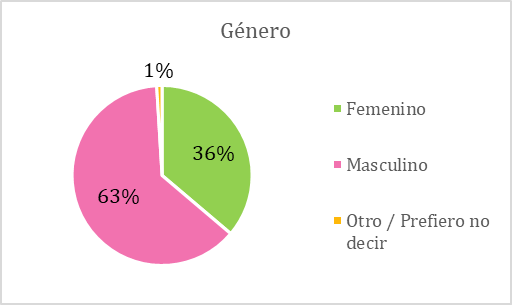
\includegraphics[width=0.5\linewidth]{figuras/encuesta_genero.png}
    \caption{Género Encuesta 2}
    \label{fig:enter-label}
\end{figure}

\begin{figure} [H]
    \centering
    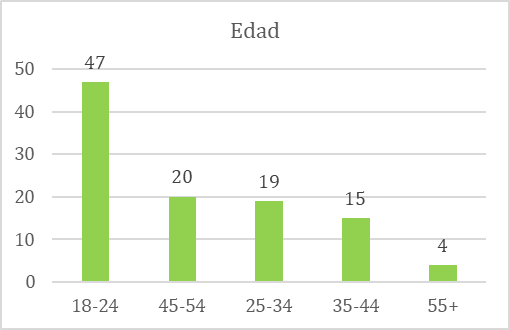
\includegraphics[width=0.5\linewidth]{figuras/encuesta_edad.png}
    \caption{Edad Encuesta 2}
    \label{fig:enter-label}
\end{figure}

La siguiente sección de la encuesta está destinada a explorar el conocimiento y la experiencia con la lengua de señas. Alrededor del 40\% de los encuestados indica conocer a alguien sordo, lo que destaca una conexión significativa con la comunidad sorda. Adicionalmente, cerca del 70\% percibe la aplicación como relevante, mostrando un interés considerable en la herramienta propuesta. Sin embargo, es notable que aproximadamente el 70\% de los participantes no están familiarizados con LENSEGUA, lo cual es entendible considerando que su reconocimiento oficial data de hace solo cuatro años. \cite{CongresoGuatemala2020}. 

\begin{figure} [H]
    \centering
    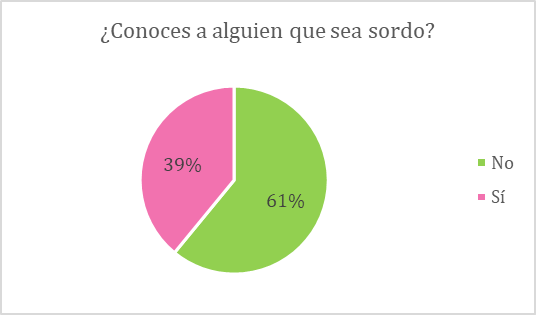
\includegraphics[width=0.5\linewidth]{figuras/conocimientoSordaEncuesta.png}
    \caption{Conocimiento Persona Sorda Encuesta 2}
    \label{fig:enter-label}
\end{figure}

\begin{figure} [H]
    \centering
    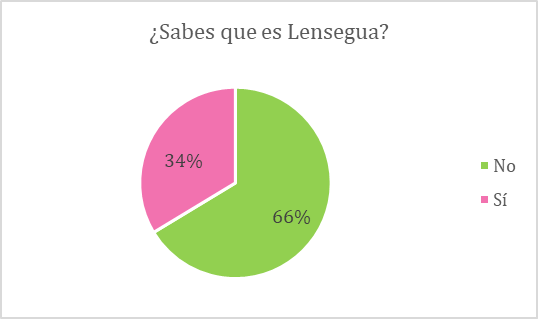
\includegraphics[width=0.5\linewidth]{figuras/conocimiento_lensegua.png}
    \caption{Conocimiento Lensegua Encuesta 2}
    \label{fig:enter-label}
\end{figure}

\begin{figure} [H]
    \centering
    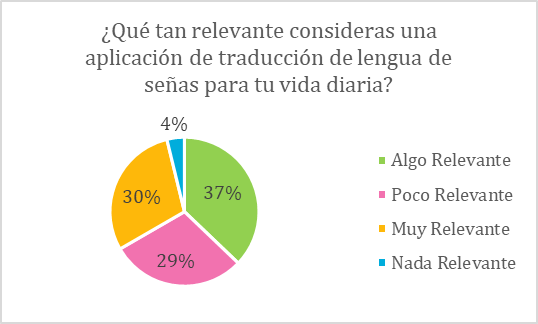
\includegraphics[width=0.5\linewidth]{figuras/relevancia_app.png}
    \caption{ Relevancia de la Aplicación Encuesta 2}
    \label{fig:enter-label}
\end{figure}


Además, se realizó un análisis comparativo entre los encuestados que conocen a personas sordas y su percepción de la relevancia de la aplicación. Los resultados muestran que aquellos familiarizados con la comunidad sorda tienden a valorar más la aplicación en comparación con quienes no tienen contacto directo con personas sordas. Este hallazgo sugiere que la experiencia personal y el conocimiento de los retos enfrentados por las personas sordas pueden influir significativamente en la percepción de la utilidad de herramientas tecnológicas como un traductor de lengua de señas.

\begin{figure} [H]
    \centering
    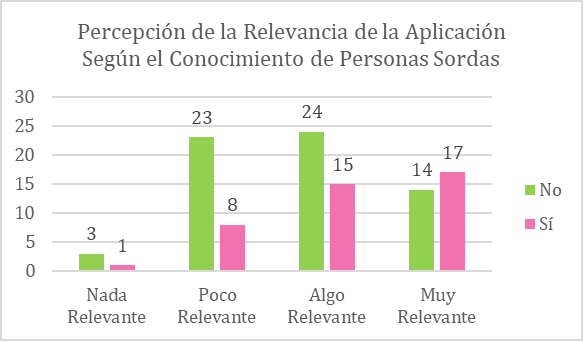
\includegraphics[width=0.5\linewidth]{figuras/relevancia_app_conocidos.png}
    \caption{Relevancia de la Aplicación para Personas con Conocidos Sordos Encuesta 2}
    \label{fig:enter-label}
\end{figure}

Para comprender mejor las estrategias de comunicación que las personas emplearían con individuos sordos, se les preguntó a los encuestados sobre sus métodos preferidos. La mayoría, casi el 60\%, optaría por el uso de mensajes escritos, mientras que un 18\% indicó que señalarían objetos para hacerse entender. Solo un 9\% consideraría usar Lensegua. Es notable que solo una minoría, aproximadamente el 10\%, expresó no saber cómo comunicarse, reflejando así el interés general por explorar formas de interacción. Algunos participantes también mencionaron la lectura de labios como alternativa, aunque es importante destacar que no todos los sordos tienen la capacidad de leer los labios.

Para profundizar en el entendimiento que tienen las personas sobre los desafíos que enfrentan los sordos, se les preguntó cuáles consideraban que eran las mayores dificultades para esta comunidad. Las respuestas revelaron una conciencia sobre la falta de inclusión y herramientas adecuadas para personas sordas, destacando cómo muchas infraestructuras y servicios en Guatemala están diseñados principalmente para oyentes. Además, se mencionaron problemas como segregación y discriminación en la sociedad, así como la escasez de enseñanza de la lengua de señas.

Entre las preocupaciones más citadas también estuvieron la ausencia de sistemas de alerta para sordos en situaciones de emergencia y barreras significativas en comunicación. Los encuestados resaltaron la existencia de prejuicios y la dificultad en la realización de tareas cotidianas y trámites, lo que contribuye al aislamiento social y a la exclusión. Esta variedad de respuestas ilustra la complejidad de los desafíos a los que se enfrentan los sordos. 

La siguiente sección de la encuesta se centró en la aplicación "Señas Chapinas", explorando las motivaciones principales para usar una herramienta de traducción de lengua de señas. Destacablemente, el 60\% de los participantes indicaron la curiosidad personal como su principal motivación. Casi la mitad de los encuestados mencionaron la comunicación con amigos o familiares sordos como un factor importante, subrayando la relevancia personal y social de la aplicación. Además, cerca del 40\% expresaron que utilizarían la aplicación para actividades voluntarias, lo que refleja su potencial utilidad en entornos de servicio comunitario. Un pequeño porcentaje citó los requerimientos laborales como motivo, sugiriendo su aplicación en contextos profesionales donde la interacción con personas sordas es frecuente. Otras respuestas revelaron usos más específicos y personales, evidenciando la diversidad de situaciones en las que los usuarios anticipan la utilidad de la aplicación.

También se indagó en que situaciones los usuarios desean emplear la aplicación ``Señas Chapinas''. Predominantemente, las actividades sociales representan el escenario más popular, con un 78.6\% de los encuestados seleccionándolo. Esto es seguido por el voluntariado y la educación, con un 67.6\% y un 49\%, respectivamente. El trabajo también es una situación comúnmente identificada, con un 40.2\% de los encuestados expresando la necesidad de utilizar la aplicación en este contexto. Estos resultados indican una fuerte preferencia por utilizar la aplicación en contextos grupales y de interacción, lo que subraya la importancia de la aplicación en facilitar la comunicación en una variedad de entornos cotidianos y profesionales.

La última sección pregunta las características más importantes en una aplicación móvil. En la última sección de la encuesta, los encuestados identificaron las características más importantes en una aplicación móvil. La facilidad de uso fue la más destacada, valorada por el 98.1\% de los participantes, seguida por la velocidad y rendimiento (61.9\%), funciones de accesibilidad (54.3\%), y diseño atractivo (46.7\%). Esto resalta la importancia de una interfaz intuitiva, un rendimiento eficiente, accesibilidad adecuada, y un diseño visualmente atractivo para los usuarios de esta aplicación. 

Finalmente se dio espacio para comentarios adicionales. En la sección final de la encuesta se exploraron las características esenciales para una aplicación de traducción de lengua de señas. La facilidad de uso fue una de las características más mencionadas, destacando su importancia para una adopción rápida por parte de los usuarios. Muchos encuestados valoraron también la velocidad y la precisión de la traducción, subrayando la necesidad de interacciones fluidas y sin errores. Algunas otras sugerencias fueron mencionadas, pero serán tomadas en cuenta para futuras mejoras, pues no están dentro del alcance del presente proyecto. 

%-------------------------------------------------------------------------------------------------------------------------------

\subsection{Colaboraciones}

Para profundizar en la comprensión de las necesidades tanto de las personas sordas como de aquellas que desean comunicarse con ellas, se decidió colaborar con varias entidades guatemaltecas dedicadas a mejorar la calidad de vida de este grupo.

En primer lugar, se participó en clases de Lengua de Señas Guatemalteca (LENSEGUA) ofrecidas por En-Señas. Esta formación permitió comprender mejor la gramática y el contexto cultural de esta lengua, elementos fundamentales para garantizar una comunicación efectiva y respetuosa.

Asimismo, la empresa ASEDES colaboró proporcionando apoyo en la realización de entrevistas y en otras actividades necesarias para el desarrollo de los diversos módulos del proyecto. Esta colaboración fue vital para asegurar que el diseño de la aplicación sea inclusivo y práctico para los usuarios.

Finalmente, la ONG Sordos Latinos de Guatemala estuvo brindando asistencia invaluable mediante el suministro de información y recomendaciones especializadas. Además, facilito entrevistas y otros recursos esenciales que enriquecieron el entendimiento y ayudaron a ajustar el proyecto para mejor atender las necesidades de la comunidad sorda en Guatemala.

%======================================================================================================
\section{DESARROLLO DE INTERFAZ Y EXPERIENCIA DE USUARIO}

\subsection{Creación de Diagrama de Afinidad}

En el desarrollo de la experiencia del usuario (UX), los diagramas de afinidad juegan un papel crucial, ya que permiten organizar y sintetizar grandes volúmenes de datos e ideas de manera visual y estructurada. Este método es especialmente valioso durante las fases iniciales de desarrollo de un proyecto, donde el entendimiento claro y la definición del problema son esenciales \cite{Maze2024}.

El proceso comienza con una lluvia de ideas, donde se generan y recopilan múltiples puntos de vista y datos sobre las necesidades y problemas de los usuarios. Esta fase es crítica, ya que establece la base de información que influirá en todas las decisiones de diseño y desarrollo subsiguientes \cite{Maze2024}.

La lluvia de ideas para Señas Chapinas organiza conceptos clave en categorías codificadas por colores, facilitando la identificación y el análisis de diversas áreas del proyecto:

\begin{itemize}
    \item \textbf{Naranja:} Define el público objetivo de la aplicación.
    \item \textbf{Amarillo:} Enumera los objetivos y metas que la aplicación pretende alcanzar.
    \item \textbf{Azul:} Destaca información crucial necesaria para el desarrollo de la aplicación.
    \item \textbf{Rojo:} Señala los problemas y desafíos que la aplicación busca resolver.
    \item \textbf{Verde:} Detalla las características y funcionalidades esperadas de la aplicación.
\end{itemize}

Este enfoque visual no solo ayuda a estructurar el proceso de planificación, sino que también asegura que todos los aspectos relevantes sean considerados, apoyando una toma de decisiones informada y alineada con las necesidades de los usuarios.

\begin{figure} [H]
    \centering
    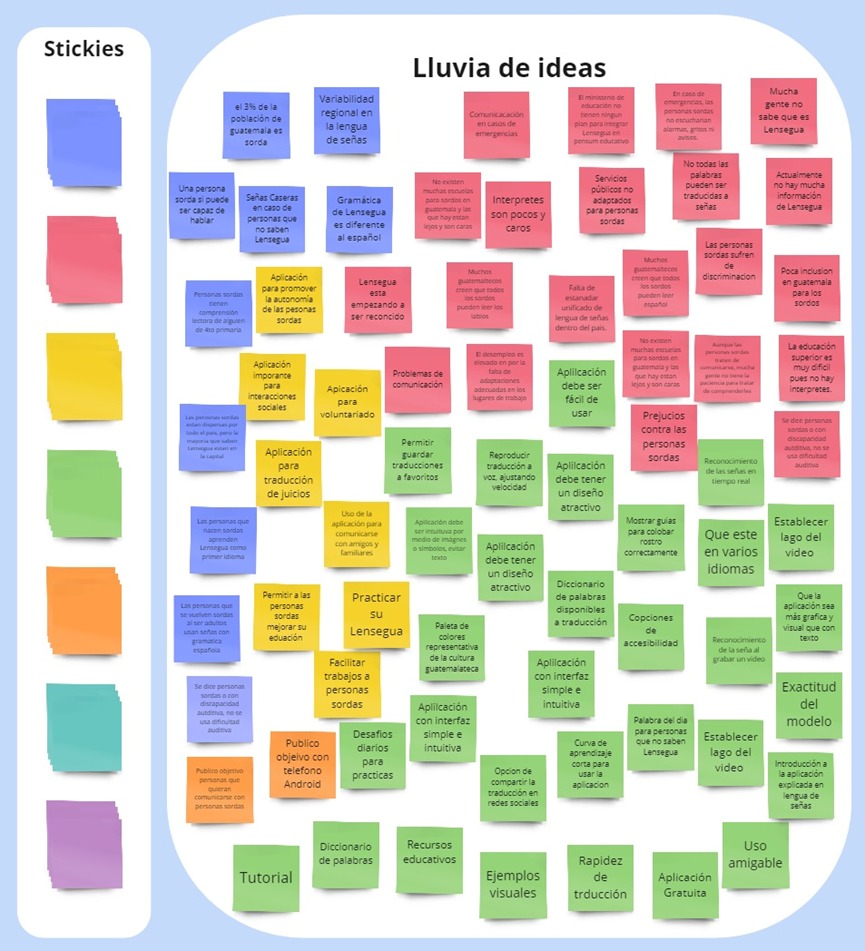
\includegraphics[width=0.75\linewidth]{figuras/lluevia_diagrama_afinidad.png}
    \caption{Lluvia de Ideas para Diagrama de Afinidad}
    \label{fig:enter-label}
\end{figure}

Posteriormente, se agrupan las ideas similares con el objetivo de identificar patrones y temas comunes. Este proceso implica organizar los datos recolectados durante la lluvia de ideas en categorías que reflejen conexiones y tendencias subyacentes. Al hacer esto, se pueden observar relaciones entre las diferentes opiniones y necesidades, facilitando la creación de soluciones más coherentes y efectivas que aborden los desafíos identificados de manera integral. Este método no solo ayuda a clarificar el alcance del proyecto, sino que también proporciona una base sólida para las decisiones de diseño y desarrollo subsiguientes, asegurando que se consideren todas las perspectivas relevantes.

\begin{figure} [H]
    \centering
    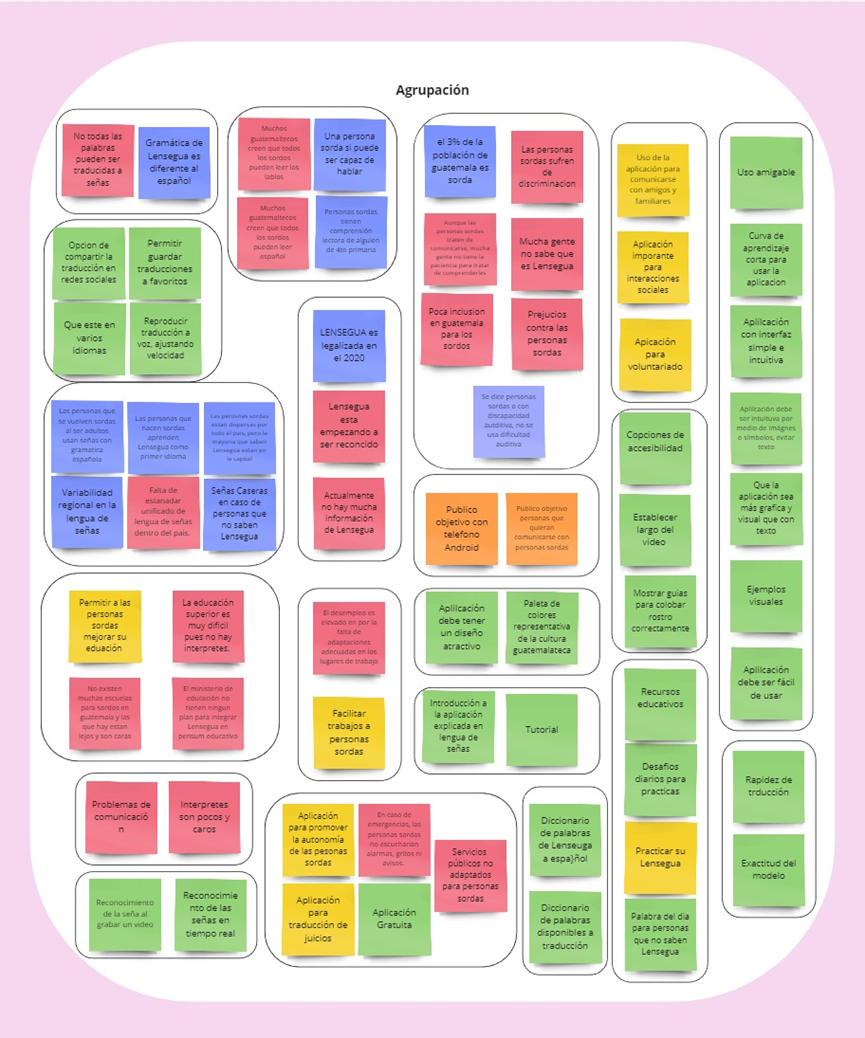
\includegraphics[width=0.75\linewidth]{figuras/agrupacion_diagrama_afinidad.png}
    \caption{Agrupación de Ideas para Diagrama de Afinidad}
    \label{fig:enter-label}
\end{figure}

Finalmente, se realiza el diagrama de afinidad, que sintetiza todas las ideas recolectadas y categorizadas previamente. Este diagrama visual, organizado por colores, facilita la interpretación de la información y permite una evaluación clara de cómo cada aspecto del proyecto interacciona y contribuye al objetivo global. Al agrupar las ideas en distintas categorías, como Público Objetivo, Problemas a Resolver, Objetivos, Escenarios de Uso, Funcionalidades a Desarrollar y Características de la Aplicación, se destaca la interconexión entre los requisitos del usuario y las soluciones propuestas.

\begin{figure} [H]
    \centering
    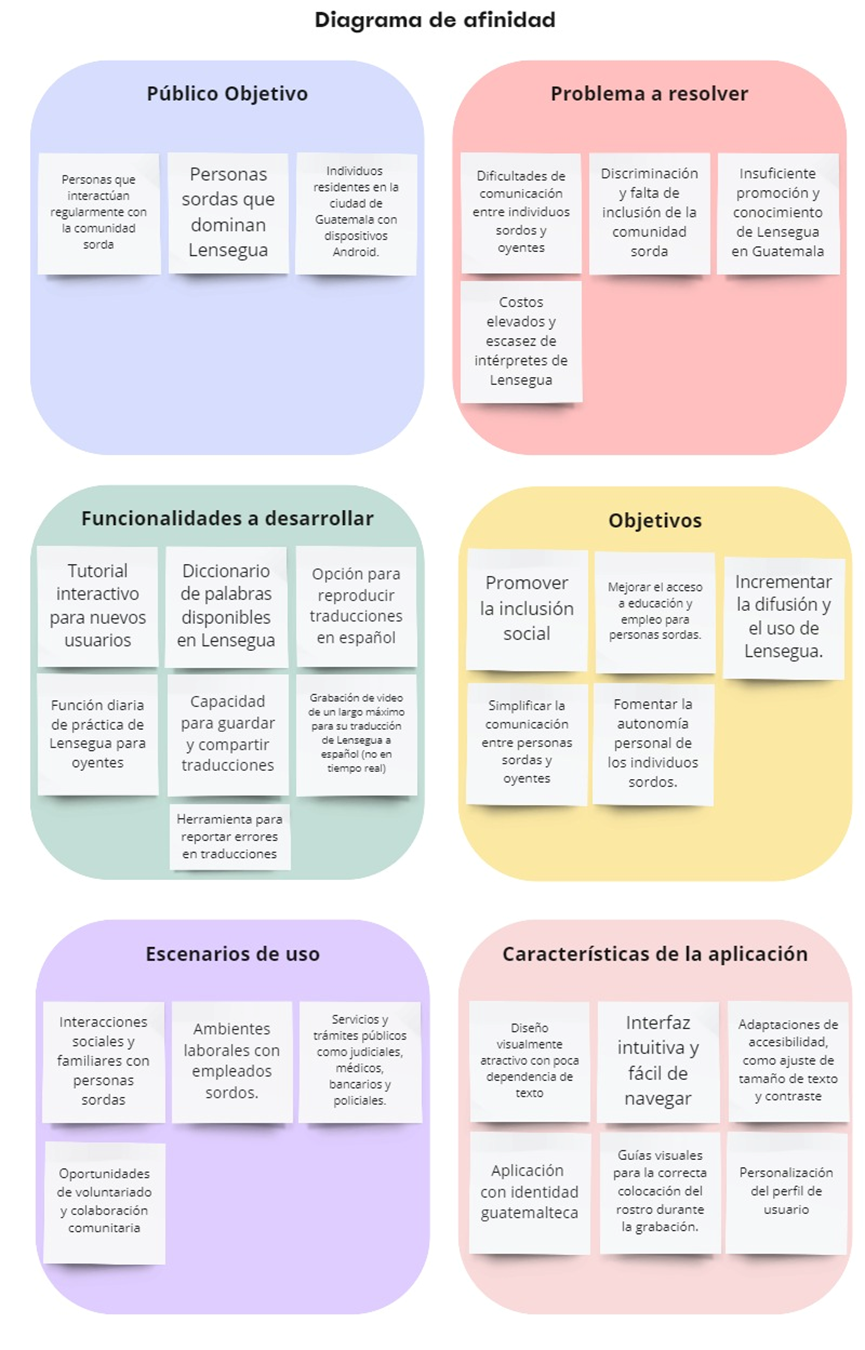
\includegraphics[width=1\linewidth]{figuras/diagrama_afinidad.png}
    \caption{Diagrama de Afinidad}
    \label{fig:enter-label}
\end{figure}

\begin{enumerate}

    \item \textbf{Público Objetivo} 
    Define a las personas que se beneficiarán directamente de la aplicación, incluyendo a aquellos que interactúan regularmente con la comunidad sorda y a las personas sordas que dominan LENSEGUA.
    \begin{itemize}
        \item Personas que interactúan regularmente con la comunidad sorda
        \item Personas sordas que dominan LENSEGUA
        \item Individuos residentes en la ciudad de Guatemala con dispositivos Android
    \end{itemize}
    
    \item \textbf{Problema a Resolver} 
    Identifica los principales desafíos que enfrenta la comunidad sorda y que la aplicación busca abordar, como las dificultades de comunicación entre sordos y oyentes, la discriminación y los altos costos de los servicios de interpretación.
    \begin{itemize}
        \item Dificultades de comunicación entre individuos sordos y oyentes
        \item Discriminación y falta de inclusión de la comunidad sorda
        \item Costos elevados y escasez de intérpretes de LENSEGUA
    \end{itemize}
    
    \item \textbf{Funcionalidades a Desarrollar} 
    Describe las características específicas que tendrá la aplicación, como un tutorial interactivo para nuevos usuarios, un diccionario de palabras en LENSEGUA, y funciones para practicar y compartir traducciones.
    \begin{itemize}
        \item Tutorial interactivo para nuevos usuarios
        \item Diccionario de palabras disponibles en LENSEGUA
        \item Función diaria de práctica de LENSEGUA para oyentes
        \item Capacidad para guardar y compartir traducciones
        \item Herramienta para reportar errores en traducciones
        \item Opción para reproducir traducciones en español
        \item Grabación de video de un largo máximo para su traducción de LENSEGUA a español (no en tiempo real)
    \end{itemize}
    
    \item \textbf{Objetivos} 
    Detalla los objetivos principales de la aplicación, como promover la inclusión social, mejorar el acceso a la educación y empleo para personas sordas, y simplificar la comunicación entre sordos y oyentes.
    \begin{itemize}
        \item Promover la inclusión social
        \item Simplificar la comunicación entre personas sordas y oyentes
        \item Mejorar el acceso a educación y empleo para personas sordas
        \item Fomentar la autonomía personal de los individuos sordos
        \item Incrementar la difusión y el uso de LENSEGUA
    \end{itemize}
    
    \item \textbf{Escenarios de Uso} 
    Enumera los diferentes contextos en los que la aplicación podría ser utilizada, incluyendo interacciones sociales, ambientes laborales, y servicios públicos como trámites médicos, bancarios y policiales.
    \begin{itemize}
        \item Interacciones sociales y familiares con personas sordas
        \item Ambientes laborales con empleados sordos
        \item Servicios y trámites públicos como judiciales, médicos, bancarios y policiales
        \item Oportunidades de voluntariado y colaboración comunitaria
    \end{itemize}
    
    \item \textbf{Características de la Aplicación} 
    Resalta aspectos del diseño y la usabilidad de la aplicación, tales como su interfaz intuitiva, el diseño visual con poca dependencia de texto y adaptaciones para accesibilidad, entre otros.
    \begin{itemize}
        \item Diseño visualmente atractivo con poca dependencia de texto
        \item Interfaz intuitiva y fácil de navegar
        \item Adaptaciones de accesibilidad, como ajuste de tamaño de texto y contraste
        \item Aplicación con identidad guatemalteca
        \item Guías visuales para la correcta colocación del rostro durante la grabación
        \item Personalización del perfil de usuario
    \end{itemize}
\end{enumerate}


\subsection{Creación de Personas}

Como parte del proceso de diseño, se han definido seis personas que representan a los usuarios finales a quienes se dirige la aplicación. 

\begin{figure} [H]
    \centering
    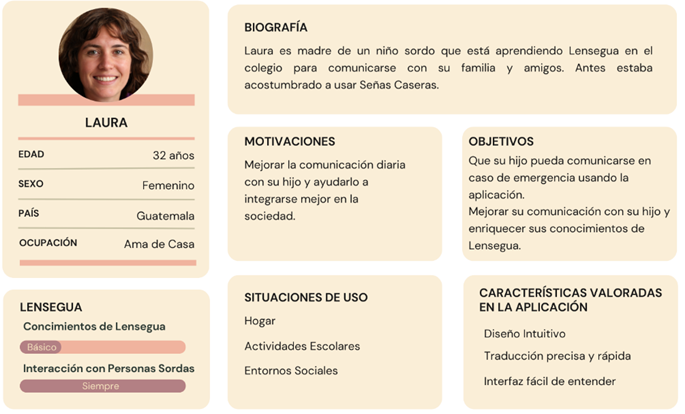
\includegraphics[width=0.8\linewidth]{figuras/persona_laura.png}
    \caption{Persona 1 - Laura}
    \label{fig:enter-label}
\end{figure}

\begin{figure} [H]
    \centering
    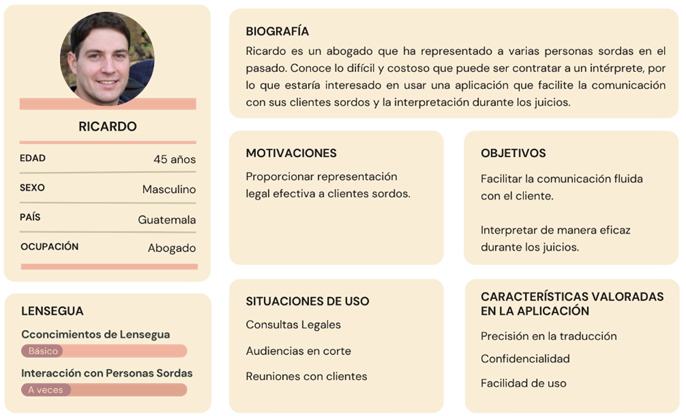
\includegraphics[width=0.8\linewidth]{figuras/ricardo_persona.png}
    \caption{Persona 2 - Ricardo}
    \label{fig:enter-label}
\end{figure}

\begin{figure} [H]
    \centering
    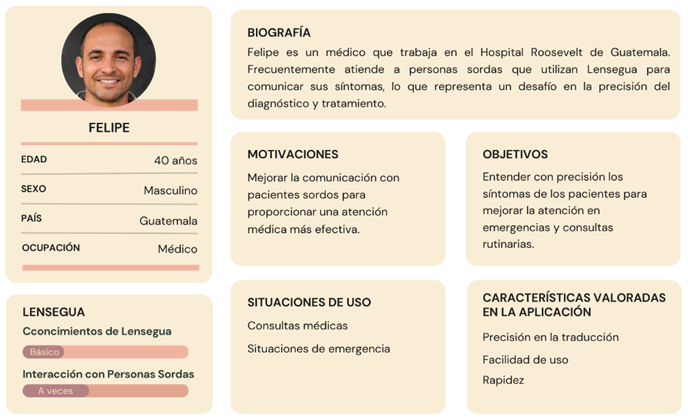
\includegraphics[width=0.8\linewidth]{figuras/felipe_persona.png}
    \caption{Persona 3 - Felipe}
    \label{fig:enter-label}
\end{figure}

\begin{figure} [H]
    \centering
    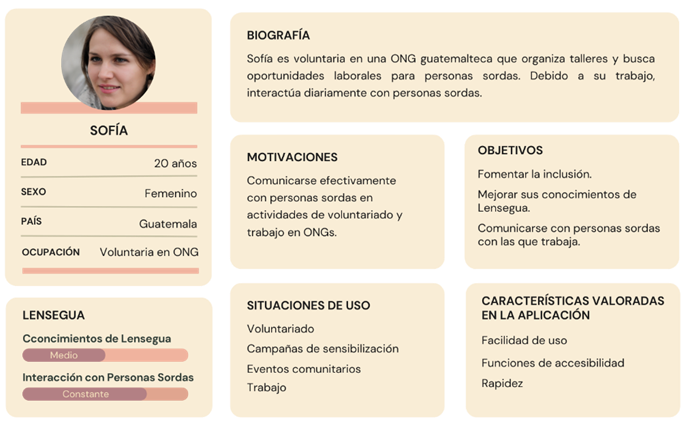
\includegraphics[width=0.8\linewidth]{figuras/sofia_persona.png}
    \caption{Persona 4 - Sofia}
    \label{fig:enter-label}
\end{figure}

\begin{figure}[H]
    \centering
    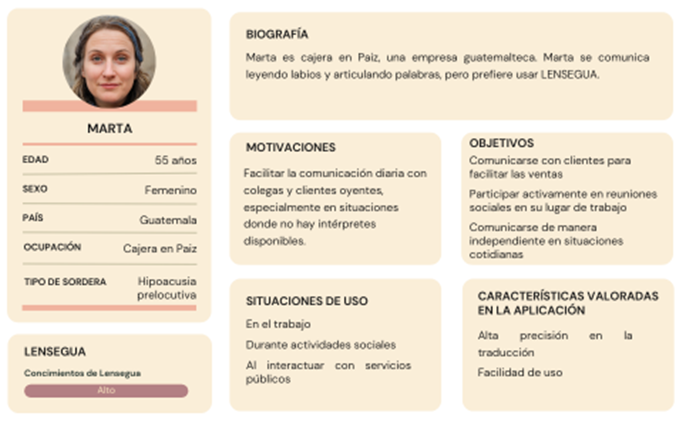
\includegraphics[width=0.8\linewidth]{figuras/marta_persona.png}
    \caption{Persona 5 - Marta}
    \label{fig:enter-label}
\end{figure}

\begin{figure} [H]
    \centering
    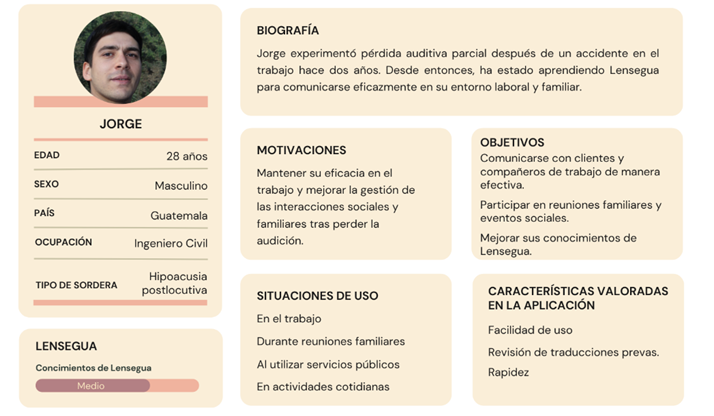
\includegraphics[width=0.8\linewidth]{figuras/jorge_persona.png}
    \caption{Persona 6 - Jorge}
    \label{fig:enter-label}
\end{figure}

% -----------------------------------------------------------------------------------------


\subsection{Creación de Mapas de Empatía}

Complementando las Personas creadas con anterioridad, se procede a crear su Mapa de Empatía respectivo para profundizar en las necesidades de los usuarios. 

\begin{figure} [H]
    \centering
    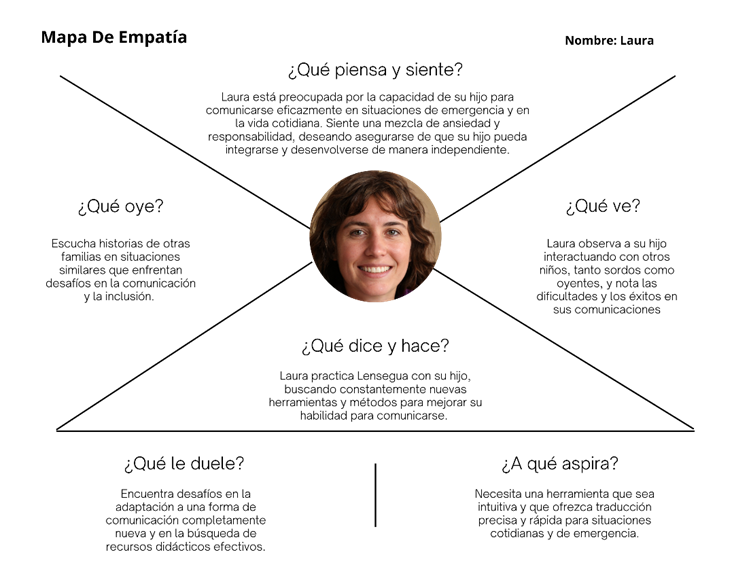
\includegraphics[width=0.9\linewidth]{figuras/mapa_empatia_laura.png}
    \caption{Mapa de Empatía - Laura}
    \label{fig:enter-label}
\end{figure}

\begin{figure} [H]
    \centering
    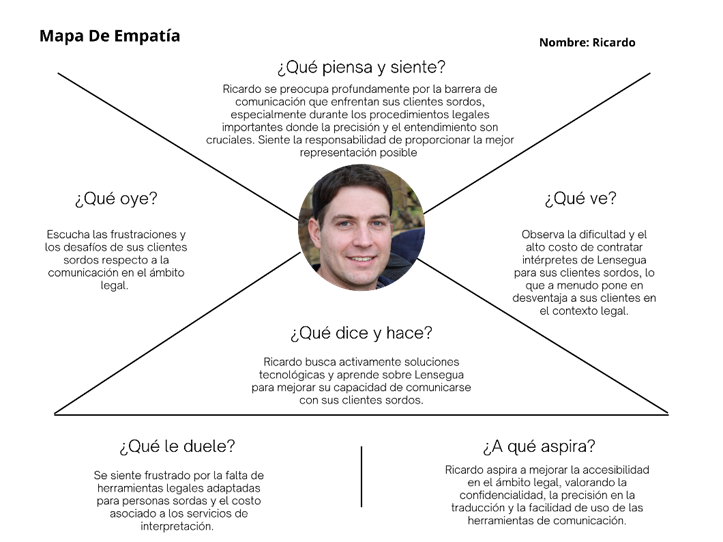
\includegraphics[width=0.9\linewidth]{figuras/mapa_empatia_ricardo.png}
    \caption{Mapa de Empatía - Ricado}
    \label{fig:enter-label}
\end{figure}

\begin{figure} [H]
    \centering
    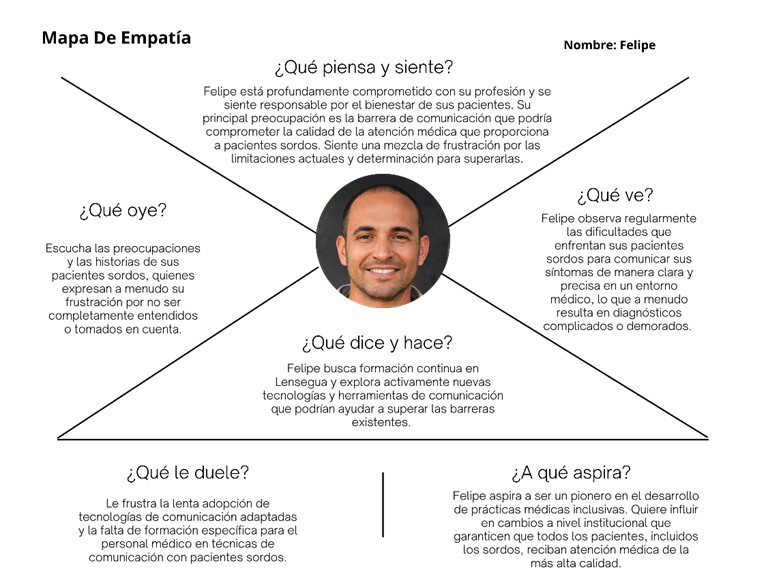
\includegraphics[width=0.9\linewidth]{figuras/mapa_empatia_felipe.png}
    \caption{Mapa de Empatía - Felipe}
    \label{fig:enter-label}
\end{figure}

\begin{figure} [H]
    \centering
    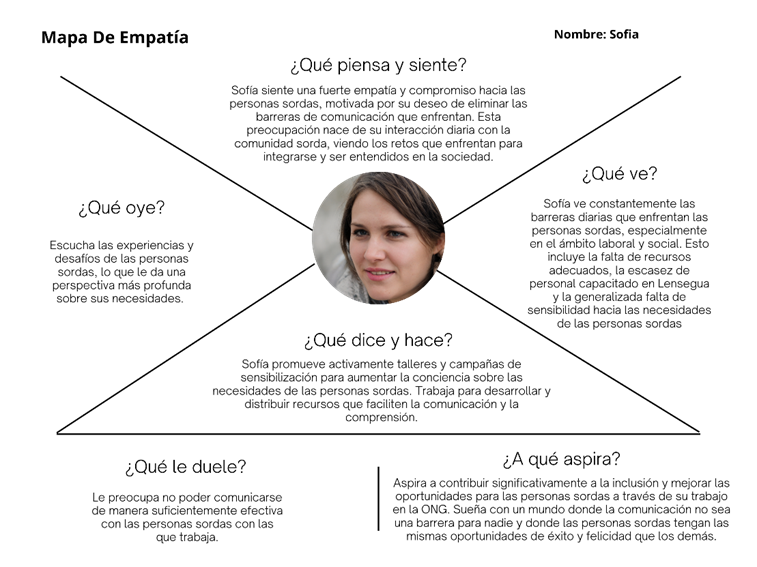
\includegraphics[width=0.9\linewidth]{figuras/mapa_empatia_sofia.png}
    \caption{Mapa de Empatía - Sofia}
    \label{fig:enter-label}
\end{figure}


\begin{figure} [H]
    \centering
    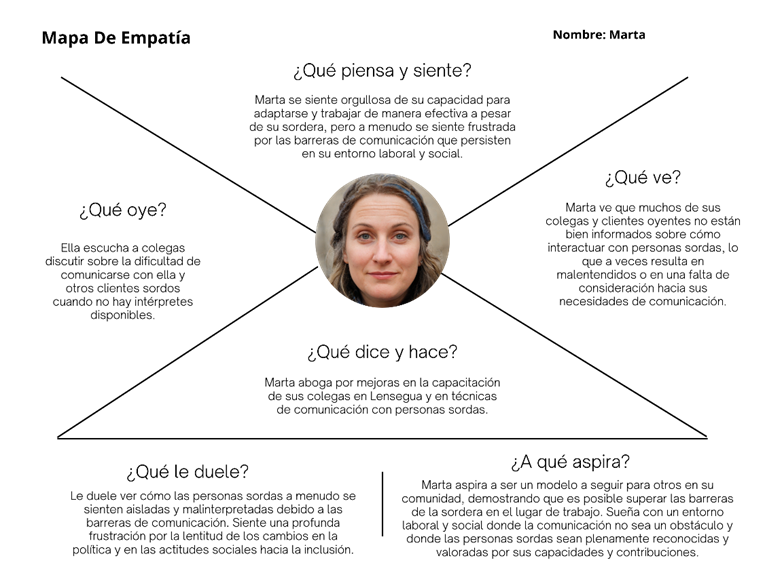
\includegraphics[width=0.9\linewidth]{figuras/mapa_empatia_marta.png}
    \caption{Mapa de Empatía - Marta}
    \label{fig:enter-label}
\end{figure}


\begin{figure} [H]
    \centering
    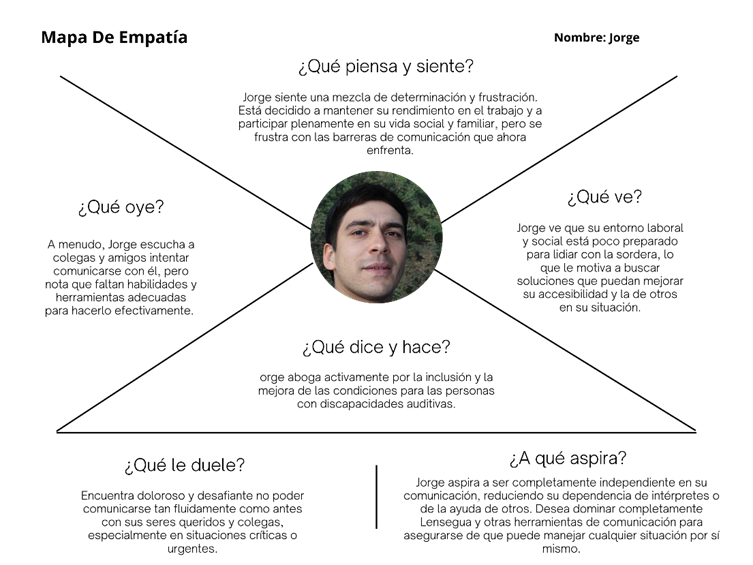
\includegraphics[width=0.9\linewidth]{figuras/mapa_empatia_jorge.png}
    \caption{Mapa de Empatía - Jorge}
    \label{fig:enter-label}
\end{figure}

% -----------------------------------------------------------------------------------------

\subsection{Planteamiento del Problema}

Inicialmente se usa Los Seis Sombreros Para Pensar, una técnica de pensamiento desarrollada por Edward de Bono en los años 80, que busca facilitar de manera creativa la resolución y el análisis de problemas desde distintos puntos de vista o perspectivas. Cada "sombrero" representa una dirección diferente del pensamiento y se identifica con un color específico \cite{Santos2024}.

\begin{figure} [H]
    \centering
    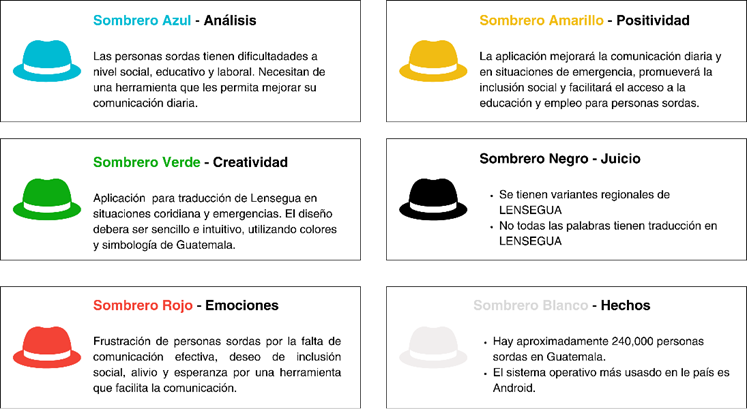
\includegraphics[width=0.8\linewidth]{figuras/sombreros.png}
    \caption{Sombreros para Pensar}
    \label{fig:enter-label}
\end{figure}


Posteriormente, se sigue el modelo W5H1 para realizar el planteamiento del problema, el cual busca ver las ideas desde varias perspectivas con el objetivo de comprender en profundidad una situación concreta \cite{Artigas2017}.

\begin{figure} [H]
    \centering
    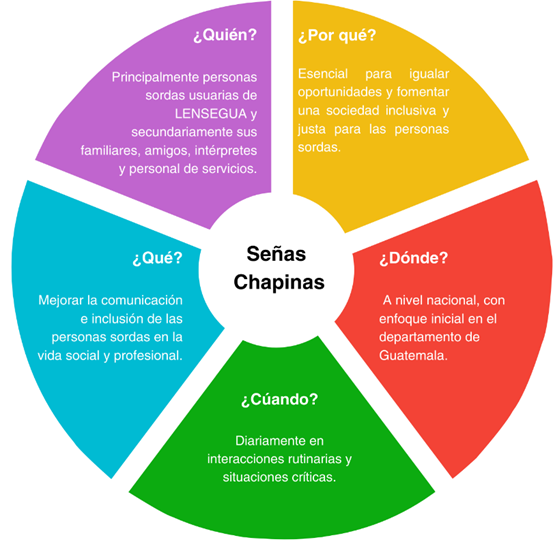
\includegraphics[width=0.6\linewidth]{figuras/w5h1.png}
    \caption{Planteamiento del Problema Señas Chapinas}
    \label{fig:enter-label}
\end{figure}

\begin{enumerate}
    \item \textbf{¿Quién?}
    \begin{enumerate}
        \item \textbf{¿A quién afecta el problema?} \\
        Afecta principalmente a personas sordas que utilizan la Lengua de Señas Guatemalteca (LENSEGUA), quienes enfrentan barreras de comunicación cotidianas.
        \item \textbf{¿Quiénes son los usuarios primarios y secundarios?}
        \begin{itemize}
            \item \textbf{Usuarios primarios:} Personas sordas, quienes dependen directamente de la comunicación efectiva para su inclusión social y profesional.
            \item \textbf{Usuarios secundarios:} Familiares, amigos, intérpretes de LENSEGUA, y personal de servicios públicos y privados que interactúan regularmente con personas sordas.
        \end{itemize}
    \end{enumerate}

    \item \textbf{¿Qué?}
    \begin{enumerate}
        \item \textbf{¿Cuáles son los límites del problema?} \\
        El problema está limitado al vocabulario esencial y de emergencia necesario para la comunicación diaria y situaciones críticas.
        \item \textbf{¿Cuál es el problema que requiere nuestra atención?} \\
        La barrera de comunicación persistente entre las personas sordas y la sociedad oyente, que limita significativamente la participación de las personas sordas en la sociedad.
        \item \textbf{¿Cuál es el objetivo final?} \\
        Facilitar la comunicación y mejorar la inclusión de la comunidad sorda en todos los aspectos de la vida social y profesional.
    \end{enumerate}

    \item \textbf{¿Cuándo?}
    \begin{enumerate}
        \item \textbf{¿Cuándo ocurre el problema?} \\
        El problema ocurre diariamente y se manifiesta en interacciones rutinarias, servicios de emergencia, entornos educativos y actividades sociales.
    \end{enumerate}

    \item \textbf{¿Dónde?}
    \begin{enumerate}
        \item \textbf{¿Dónde ocurre el problema?} \\
        El problema ocurre a lo largo de Guatemala, con un enfoque inicial en el departamento de Guatemala, debido a las variaciones dialectales de LENSEGUA en diferentes regiones.
        \item \textbf{¿Dónde se necesita enfocar más?} \\
        El enfoque inicial será en áreas urbanas donde la densidad de población y la diversidad de servicios intensifican las necesidades de comunicación efectiva.
    \end{enumerate}

    \item \textbf{¿Por qué?}
    \begin{enumerate}
        \item \textbf{¿Por qué es importante arreglar el problema?} \\
        Es importante abordar este problema para garantizar que las personas sordas en Guatemala tengan igualdad de oportunidades en su integración y participación en todos los aspectos de la vida social y profesional. Mejorar la comunicación no solo incrementa la autonomía y el bienestar de las personas sordas, sino que también contribuye a una sociedad más inclusiva y justa, donde todos los ciudadanos pueden contribuir plenamente y sin barreras.
    \end{enumerate}
\end{enumerate}

% -----------------------------------------------------------------------------------------

\subsection{Creación de Mapas de Experiencia del Cliente}

El objetivo de estos mapas es entender y abordar las necesidades y los problemas del cliente en cada etapa del proceso, identificando oportunidades para mejorar la experiencia del cliente y asegurando que cada punto de contacto con el producto sea positivo y coherente. Esto permite ver dónde se encuentran los puntos de dolor y adoptar mejoras para ofrecer una experiencia más satisfactoria y efectiva \cite{Hamond2024}.

Los mapas realizados incluyen los flujos principales a realizar dentro de la aplicación: Primera vez usando la aplicación como usuario, para identificar puntos de mejora con el primer contacto con los usuarios; grabación de videos, para identificar como debe actual la aplicación para que la funcionalidad sea sencilla; guardado de video, para analizar como debe realizarse el proceso; reporte de traducción errónea, para facilitar una manera de que los usuarios puedan ayudar a mejorar la aplicación; diccionario de palabras, para entender de qué manera los usuario usaría esta herramienta; y finalmente el reto diario, para identificar puntos de dolor en esta actividad. 

\begin{figure} [H]
    \centering
    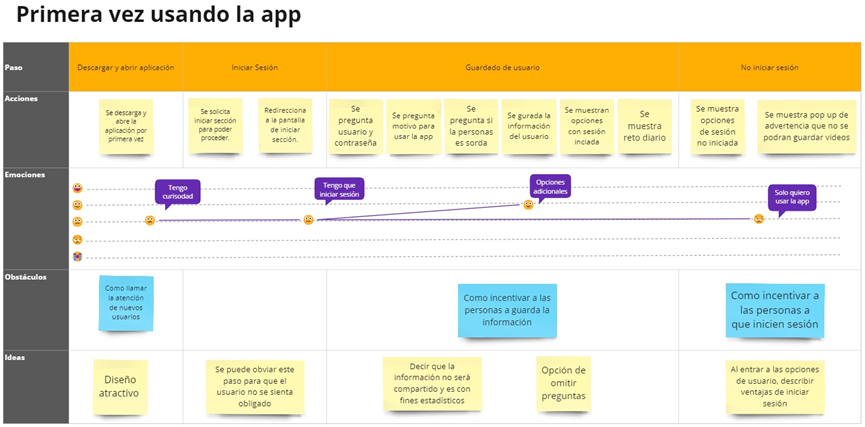
\includegraphics[width=1\linewidth]{figuras/mapa_exp1.png}
    \caption{Primera vez usando la app}
    \label{fig:enter-label}
\end{figure}

\begin{figure} [H]
    \centering
    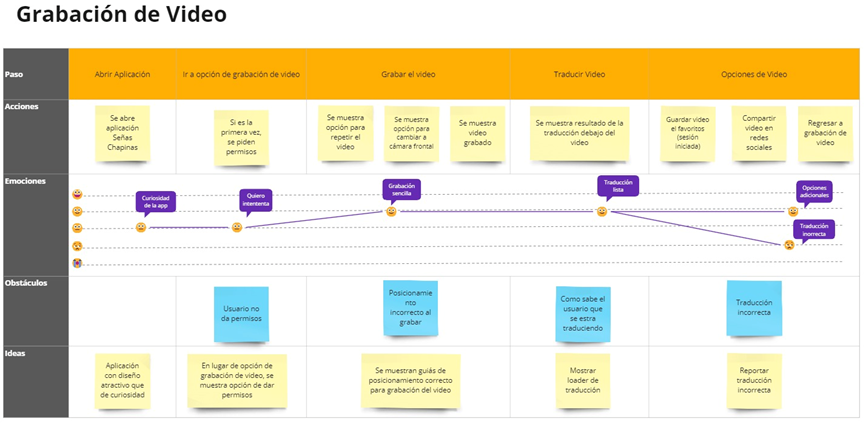
\includegraphics[width=1\linewidth]{figuras/mapa_exp2.png}
    \caption{Grabación de video}
    \label{fig:enter-label}
\end{figure}


\begin{figure} [H]
    \centering
    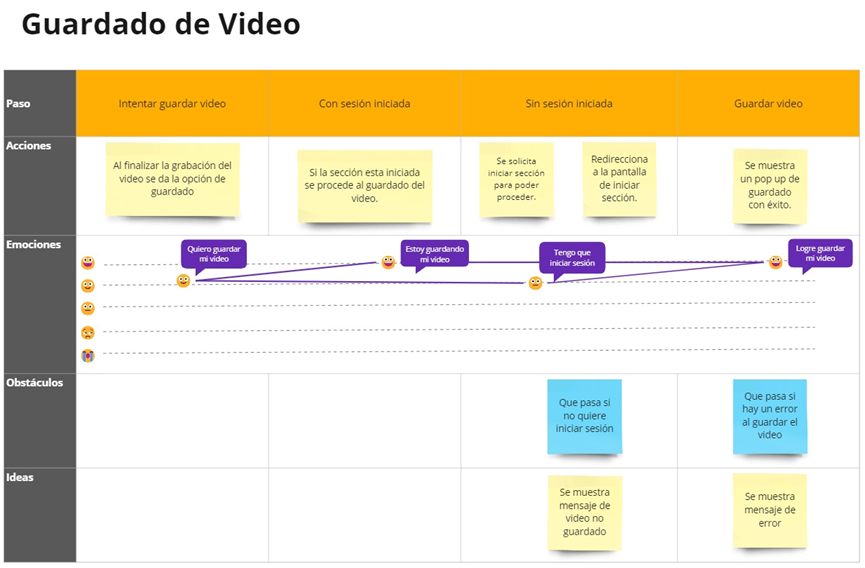
\includegraphics[width=1\linewidth]{figuras/mapa_exp3.png}
    \caption{Guardando Video}
    \label{fig:enter-label}
\end{figure}

\begin{figure} [H]
    \centering
    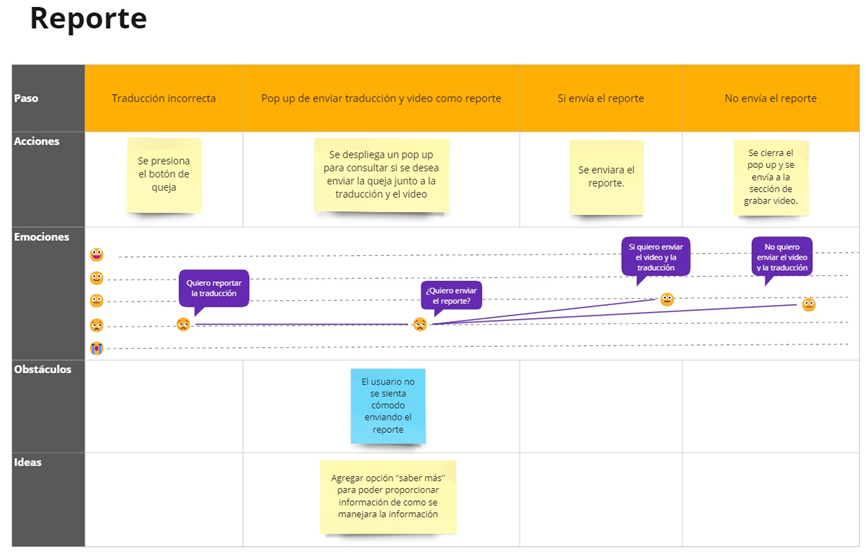
\includegraphics[width=1\linewidth]{figuras/mapa_exp4.png}
    \caption{Reporte}
    \label{fig:enter-label}
\end{figure}

\begin{figure} [H]
    \centering
    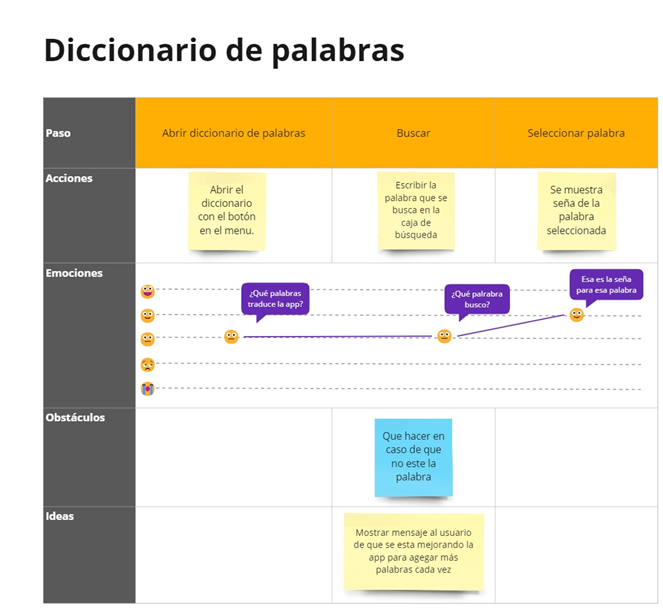
\includegraphics[width=0.8\linewidth]{figuras/mapa_exp5.png}
    \caption{Diccionario de palabras}
    \label{fig:enter-label}
\end{figure}

\begin{figure} [H]
    \centering
    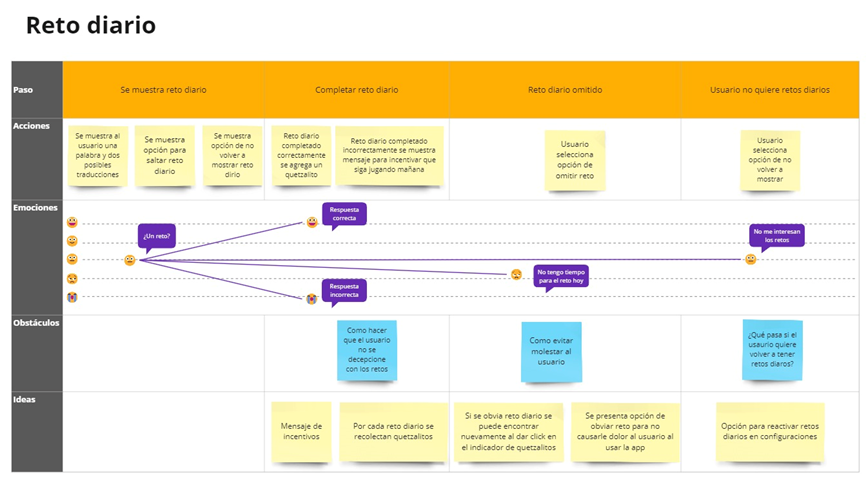
\includegraphics[width=1\linewidth]{figuras/mapa_exp6.png}
    \caption{Reto diario}
    \label{fig:enter-label}
\end{figure}

% -----------------------------------------------------------------------------------------

\subsection{Mapa de Sitio}

Los mapas de sitio proporcionados visualizan la estructura y navegación de la aplicación ``Señas Chapinas'', facilitando un entendimiento claro de las funcionalidades disponibles para los usuarios en diferentes estados.

\begin{itemize}
    \item \textbf{Pantalla para Grabar Video}: Permite a los usuarios grabar un video que luego puede ser traducido a LENSEGUA o repetido. 
    \begin{itemize}
        \item \textbf{Compartir video y traducción}: Luego de traducir el video, se puede compartir el video y su traducción.
        \item \textbf{Reportar traducción incorrecta}: Si la traducción es incorrecta, los usuarios pueden reportar errores.
        \item \textbf{Guardar video}: Los usuarios con sesión iniciada pueden guardar traducciones realizadas para consultarlas nuevamente.
    \end{itemize}
    \item \textbf{Diccionario de palabras}: Misma funcionalidad que en el estado sin sesión iniciada.
    \item \textbf{Cuenta}: Acceso a opciones de inicio de sesión y configuración general de la app.
    \begin{itemize}
        \item \textbf{Información del usuario}: Muestra los detalles del usuario registrado.
        \item \textbf{Racha de retos diarios}: Muestra el progreso del usuario en retos diarios de aprendizaje.
        \item \textbf{Videos Guardados}: Acceso a videos que el usuario ha decidido guardar.
        \begin{itemize}
            \item Al seleccionar un video guardado se acceden a las mismas opciones de video traducido (compartir, reportar o grabar video).
        \end{itemize}
        \item \textbf{Configuración / Sobre la app / Ayuda}: Opciones para mejorar la experiencia del usuario en la aplicación.
        \item \textbf{Cerrar Sesión}: Permite al usuario salir de su cuenta.
    \end{itemize}
\end{itemize}

\begin{figure} [H]
    \centering
    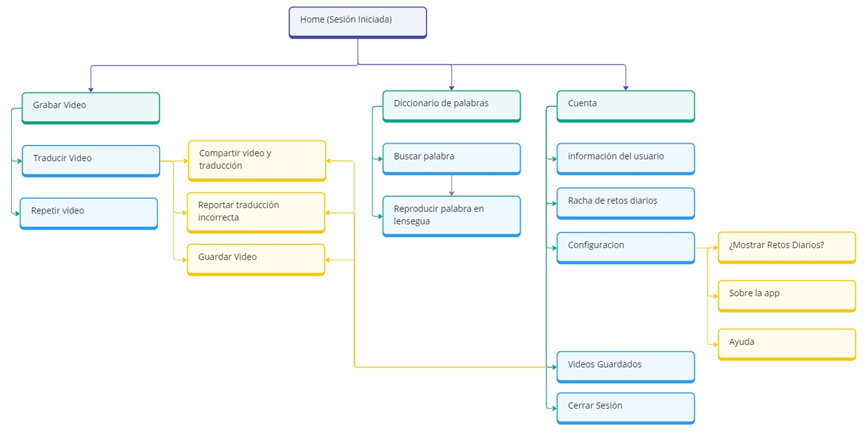
\includegraphics[width=1\linewidth]{figuras/mapa_sitio.png}
    \caption{Mapa de Sitio}
    \label{fig:enter-label}
\end{figure}

% -----------------------------------------------------------------------------------------

\subsection{Flujo de Usuarios}

En el diseño de UX, un flujo de usuarios es una representación visual de los pasos que un usuario sigue dentro de una aplicación para alcanzar un objetivo específico. Esto incluye todas las acciones, decisiones y procesos desde el punto de entrada hasta la salida \cite{Adobe2022}.

Para crear un flujo de usuarios efectivo, es crucial seguir algunos pasos detallados:

\begin{enumerate}
    \item \textbf{Comprender el viaje del cliente}: Con la información recopilada en las Personas, los mapas de empatía y los mapas de la experiencia del cliente, se identificaron las necesidades, motivaciones y comportamientos de los usuarios \cite{Adobe2022}.
    
    \item \textbf{Identificar y alinear los objetivos}: Cada sección de la aplicación debe tener un objetivo claro que puede diferir de los objetivos del usuario. Por lo tanto, es esencial identificar lo que los usuarios buscan lograr y alinear los objetivos de la aplicación con los de ellos para asegurar que el flujo de usuario los guíe efectivamente hacia acciones deseadas \cite{Adobe2022}.
    
    \item \textbf{Decidir la información que necesitan los usuarios}: Basado en las Personas y los mapas del viaje del cliente, se definen los pasos necesarios que los usuarios deben seguir dentro del flujo, abordando sus puntos de dolor y proporcionando la información que buscan en cada etapa \cite{Adobe2022}.
    
    \item \textbf{Visualizar el flujo}: Finalmente, se visualiza y mapea el flujo utilizando formas para comunicar los diferentes caminos y decisiones en un flujo de usuarios \cite{Adobe2022}.
    \begin{itemize}
        \item Los óvalos representan el inicio y el final de un flujo de usuarios.
        \item Los rectángulos simbolizan un paso del proceso, una página de la aplicación.
        \item Las flechas conectan las formas y muestran la dirección del camino del usuario.
        \item Los diamantes representan decisiones que los usuarios toman en cada paso.
        \item Los paralelogramos indican dónde el usuario debe ingresar algo.
        \item El rectángulo redondeado simboliza mensajes al usuario o notificaciones dentro de la aplicación.
    \end{itemize}
    
    \item \textbf{Obtener retroalimentación}: Para mejorar el flujo de usuarios, se comparte con partes interesadas para identificar posibles fricciones en el flujo y encontrar mejores formas de agilizar y mejorar la experiencia del usuario \cite{Adobe2022}.
\end{enumerate}

El primer Flujo de Usuario realizado es para Marta. Marta es sorda profunda y trabaja como cajera por lo que desea ofrecer sus productos de caja para obtener comisiones. Para ello graba un video y reproduce el audio de la traducción. 

\begin{figure} [H]
    \centering
    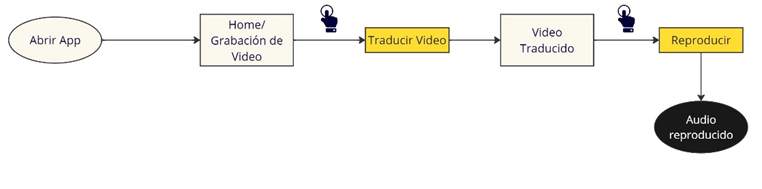
\includegraphics[width=1\linewidth]{figuras/flujo_usuario1.png}
    \caption{Grabar video}
    \label{fig:enter-label}
\end{figure}

Posteriormente se da cuenta que puede guardar el video para usarlo múltiples veces.

\begin{figure}  [H]
    \centering
    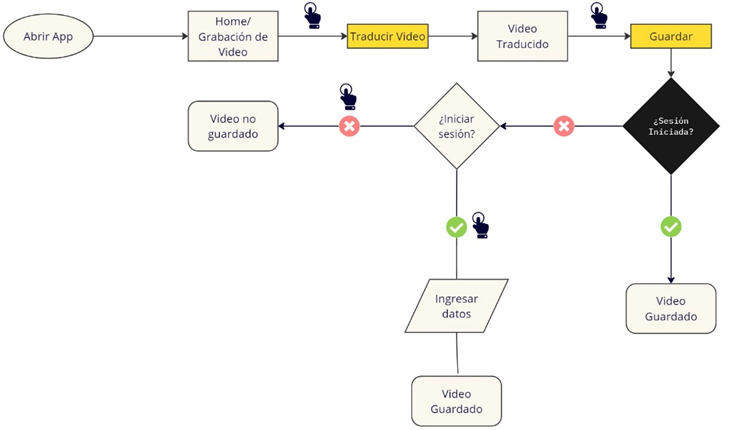
\includegraphics[width=1\linewidth]{figuras/flujo_usuario2.png}
    \caption{Guardar Video}
    \label{fig:enter-label}
\end{figure}

\begin{figure} [H]
    \centering
    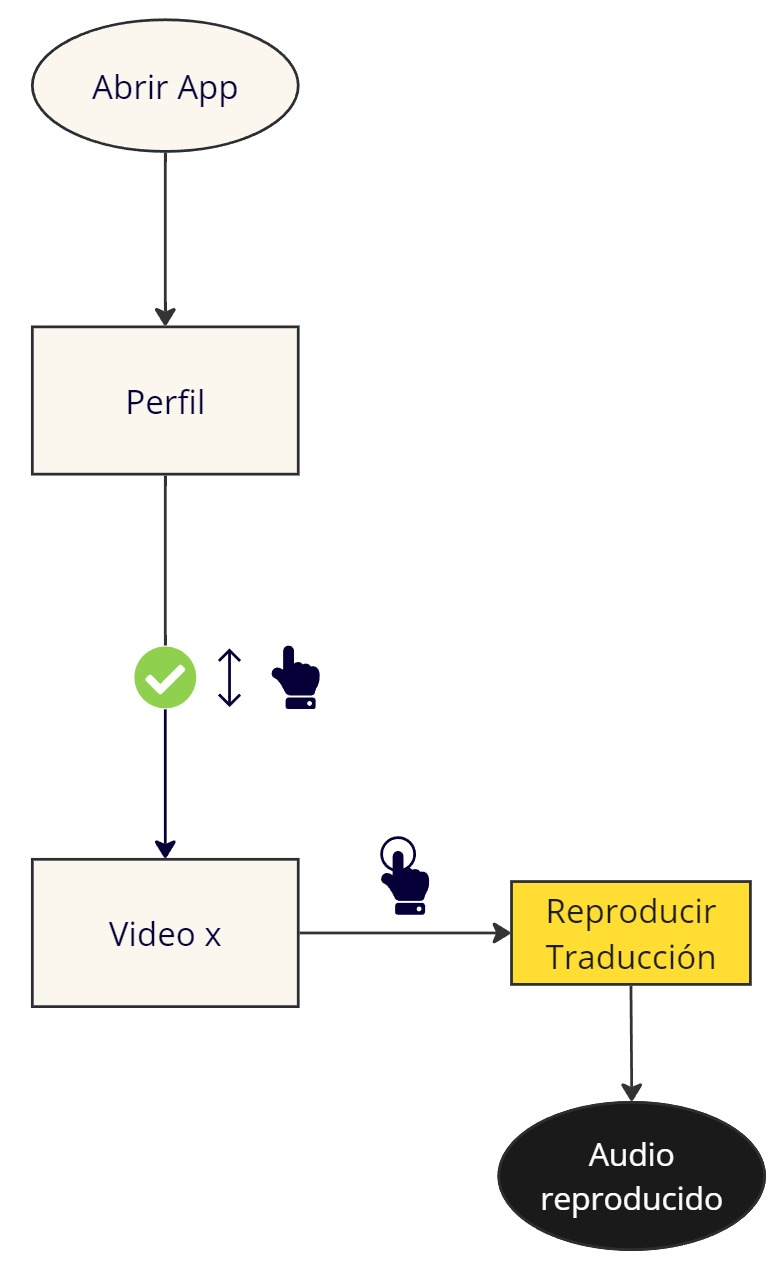
\includegraphics[width=0.3\linewidth]{figuras/flujo_usuario3.jpg}
    \caption{Abrir Video Guardado}
    \label{fig:enter-label}
\end{figure}


Por otra parte, Ricardo tiene sesiones constantemente con sus clientes, por lo que graba y guarda videos constantemente. Adicionalmente, le gusta repetir sus videos para que queden a su gusto. 

\begin{figure} [H]
    \centering
    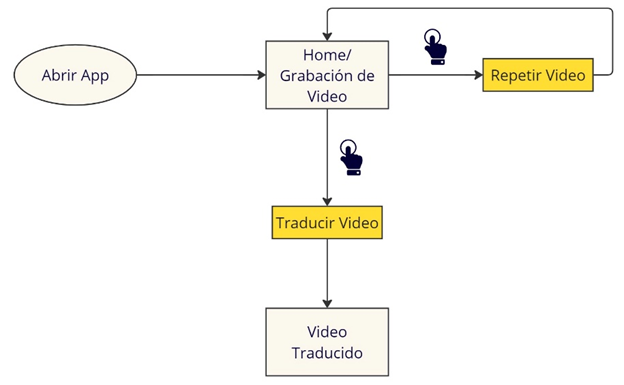
\includegraphics[width=0.7\linewidth]{figuras/flujo_usuario4.png}
    \caption{Repertir grabación de video}
    \label{fig:enter-label}
\end{figure}


Laura a su vez, al ser madre de un hijo sordo está aprendiendo LENSEGUA. Por eso le parece importante completar los retos diarios. 


\begin{figure} [H]
    \centering
    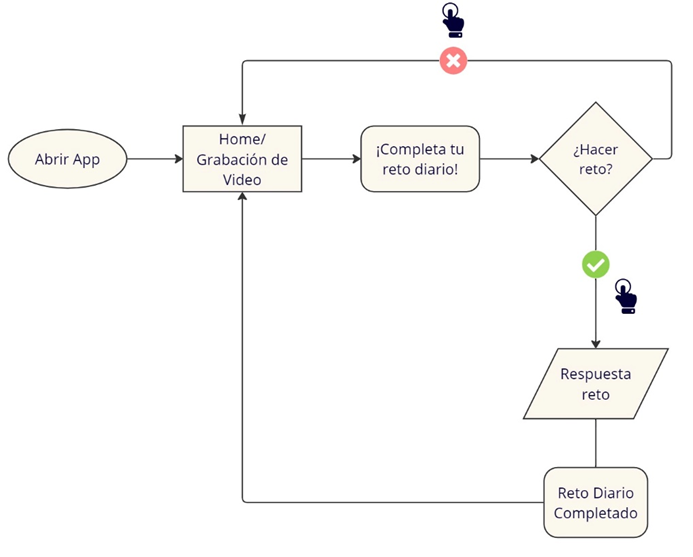
\includegraphics[width=0.75\linewidth]{figuras/flujo_usuario6.png}
    \caption{Completar reto}
    \label{fig:enter-label}
\end{figure}


Jorge por su parte, al estar aprendiendo LENSEGUA considera muy importante tener traducciones precisas. Por ello al obtener un resultado incorrecto en su traducción, rápidamente reporta el problema.

\begin{figure} [H]
    \centering
    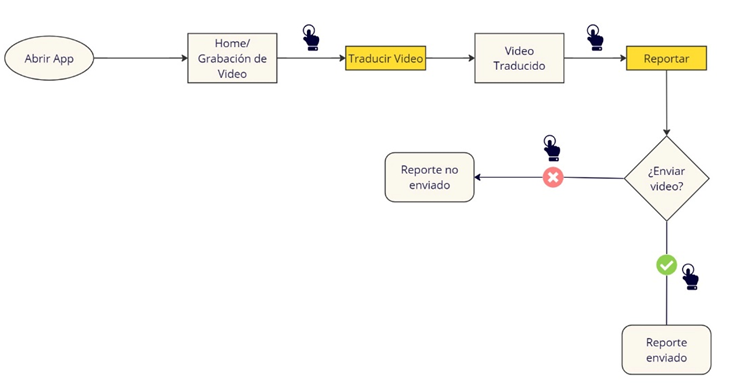
\includegraphics[width=1\linewidth]{figuras/flujo_usuario7.png}
    \caption{Reportar traducción}
    \label{fig:enter-label}
\end{figure}


Sofía es voluntaria por lo que al tener contacto con la comunidad sorda, despertó su interés por aprender LENSEGUA. Por eso accede al diccionario para mejorar su vocabulario. 


\begin{figure} [H]
    \centering
    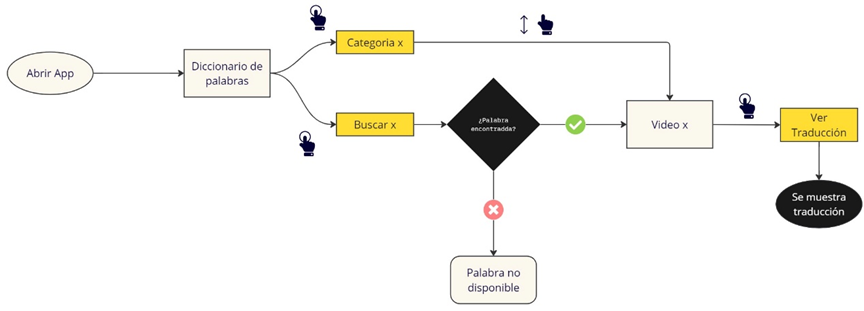
\includegraphics[width=1\linewidth]{figuras/flujo_usuario8.png}
    \caption{Diccionario}
    \label{fig:enter-label}
\end{figure}


% -----------------------------------------------------------------------------------------

\subsection{Estructura Alámbrica}

Un \textit{Wireframe} o Estructura Alámbrica, es un esquema visual que representa la estructura básica de una aplicación, mostrando el diseño y la disposición de los elementos clave sin entrar en detalles sobre el estilo gráfico o contenido final. Los Wireframes utilizan formas simples como rectángulos, líneas y texto básico para indicar elementos como encabezados, párrafos, imágenes y botones \cite{Rees2024}.

\newpage
\begin{itemize}
    \item Baja Fidelidad

        \begin{figure} [H]
            \centering
            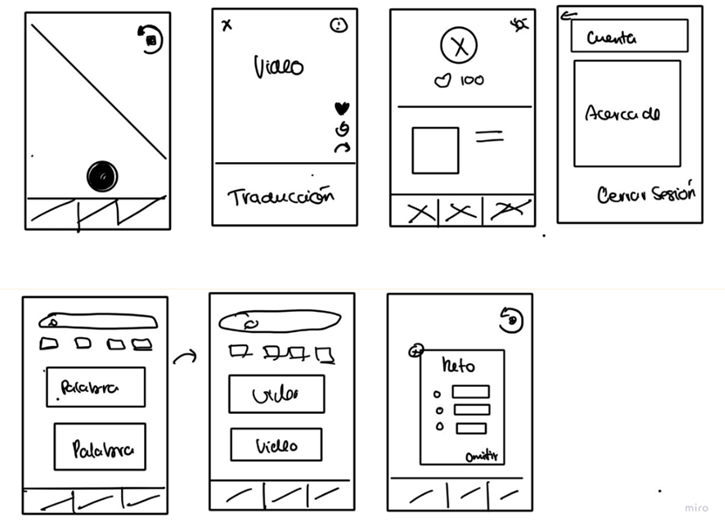
\includegraphics[width=0.8\linewidth]{figuras/wireframe_baja.png}
            \caption{Wireframe bajo nivel}
            \label{fig:enter-label}
        \end{figure}
    
    \item Media Fidelidad

        \begin{figure} [H]
            \centering
            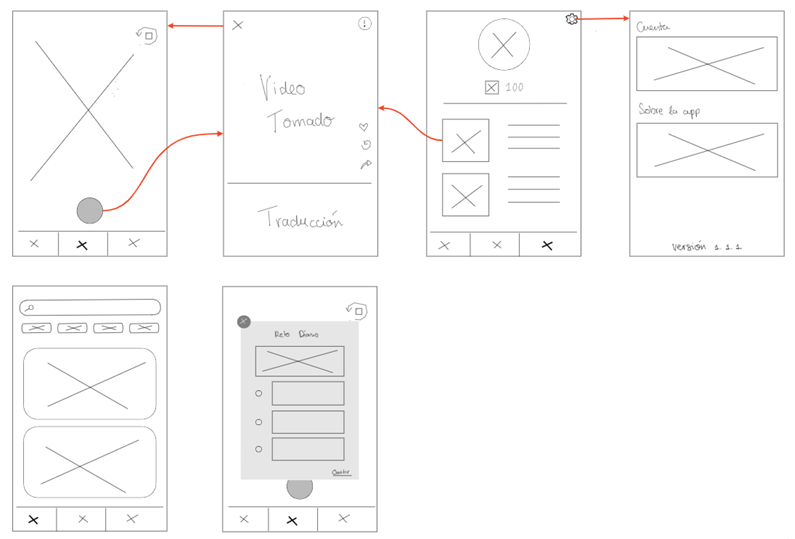
\includegraphics[width=0.9\linewidth]{figuras/wireframe_media.png}
            \caption{Wireframe nivel medio}
            \label{fig:enter-label}
        \end{figure}

    \newpage
    \item Alta Fidelidad

        \begin{figure}[H]
            \centering
            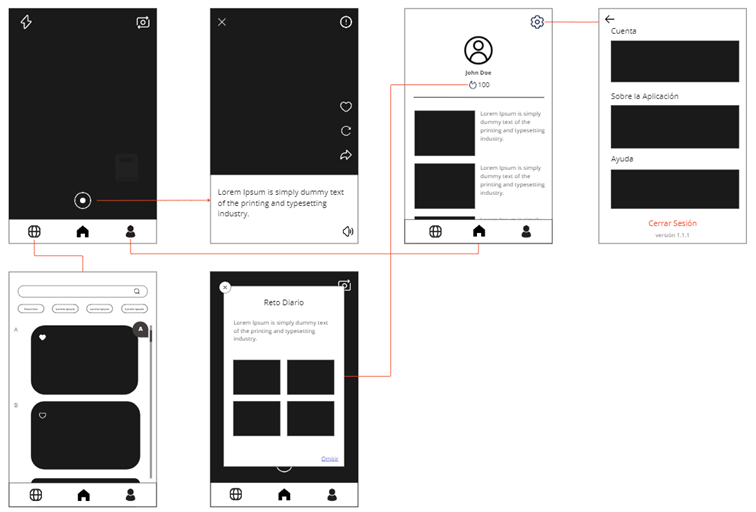
\includegraphics[width=1\linewidth]{figuras/fireframe_alta1.png}
            \caption{Wireframe alto nivel}
            \label{fig:enter-label}
        \end{figure}
    
\end{itemize}

Al llegar a este punto del desarrollo de la interfaz y experiende de usuario de hace\textbf{ una primera validación con usuarios finales}. Se tuvo una reunión con varias personas de \textit{En-Señas} pertencientes tanto a la comunidad sorda como a la comunidad oyente. Tomando en cuenta los comentarios y sugerencias de esta validación, se hicieron algunas mejoras.

\begin{itemize}
    \item 
    Se ha añadido una nueva pantalla denominada ``Traducció'' cuyo propósito es permitir que las personas escriban frases en gramática LENSEGUA, que luego son traducidas a gramática española. Esta funcionalidad fue desarrollada en respuesta a los comentarios sobre cómo las personas sordas utilizan herramientas como \textit{ChatGPT} para mejorar su gramática escrita. Es importante destacar que, según los entrevistados, el nivel de comprensión lectora de una persona sorda promedio equivale aproximadamente al de un niño en tercer grado de primaria. Por lo tanto, esta herramienta no solo busca mejorar las habilidades de escritura de las personas sordas, sino también incrementar su confianza al comunicarse por escrito.
    
    \item
    En la pantalla del usuario, se han añadido ahora opciones para marcar como favoritos no solo vídeos sino también traducciones.
    
    \item 
    En el diccionario, se ha implementado que las tarjetas se vuelvan interactivas, funcionando como \textit{flashcards}. Cada tarjeta muestra, por un lado, la palabra acompañada de una imagen, y por el otro, la señal correspondiente. La inclusión de imágenes fue una recomendación de intérpretes, quienes destacaron que las personas sordas tienden a ser muy visuales y que estas representaciones facilitarían significativamente su comprensión de las palabras.
    
\end{itemize}

Teniendo en cuenta estos comentarios y otras sugerencias menores, se realizaron diversas mejoras que culminaron en la creación de un nuevo wireframe de alto nivel.

\begin{figure} [H]
    \centering
    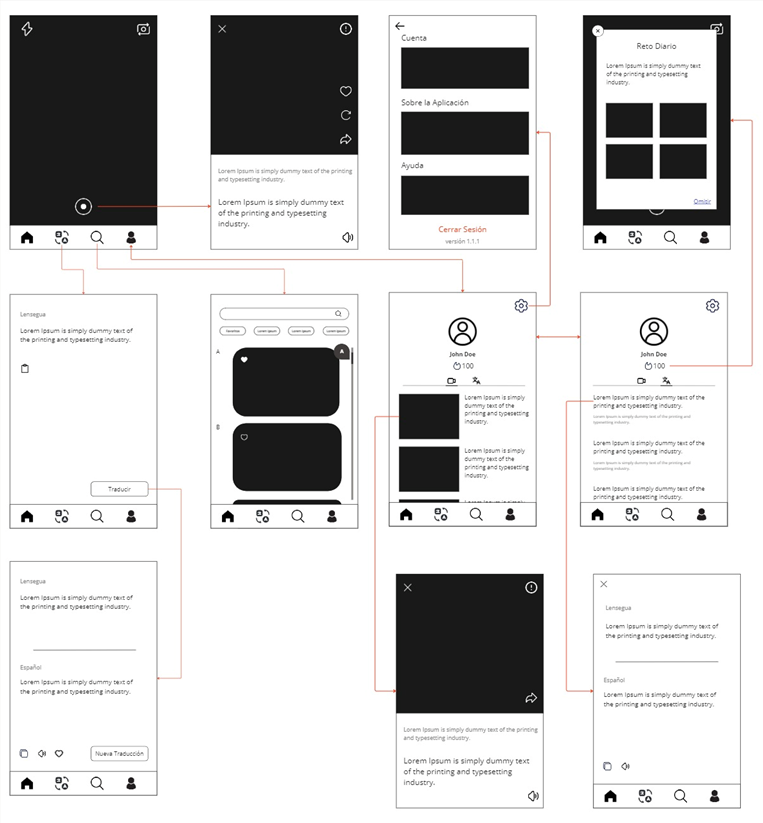
\includegraphics[width=1\linewidth]{figuras/wireframe_alto2.png}
    \caption{Wireframe alto nivel luego de retroalimentación}
    \label{fig:enter-label}
\end{figure}

Se consolida entonces la siguiente estructura para la aplicación:

\begin{enumerate}
    \item \textbf{Pantalla 1: Home}
    \begin{itemize}
        \item \textbf{Función Principal:} Pantalla de inicio.
        \item \textbf{Elementos:}
        \begin{itemize}
            \item Botón principal para grabar video.
            \item Botones adicionales para funcionalidades como cambiar cámara, activar flash, etc.
            \item Barra de navegación en la parte inferior con cuatro íconos para acceder a las cuatro secciones de la aplicación.
        \end{itemize}
    \end{itemize}

    \item \textbf{Pantalla 2: Traducción de video}
    \begin{itemize}
        \item \textbf{Función Principal:} Mostrar el video grabado junto con su traducción.
        \item \textbf{Elementos:}
        \begin{itemize}
            \item Área de reproducción del video.
            \item Traducción del video en la parte inferior.
            \item Botones para agregar a favoritos, compartir, repetir el video, reportar errores en la traducción y cerrar traducción.
        \end{itemize}
    \end{itemize}

    \item \textbf{Pantalla 3: Traducción de LENSEGUA a español}
    \begin{itemize}
        \item \textbf{Función Principal:} Traducir de gramática del sordo a español.
        \item \textbf{Elementos:}
        \begin{itemize}
            \item Sección de LENSEGUA para escribir o pegar texto.
            \item Sección de traducción al español para copiar, escuchar o guardar la traducción.
            \item Botón para traducir/nueva traducción.
        \end{itemize}
    \end{itemize}

    \item \textbf{Pantalla 4: Perfil de usuario}
    \begin{itemize}
        \item \textbf{Función Principal:} Mostrar la información del perfil del usuario.
        \item \textbf{Elementos:}
        \begin{itemize}
            \item Ícono de perfil y nombre del usuario.
            \item Contador de días de racha de desafíos completados.
            \item Lista de videos favoritos con sus respectivas traducciones.
            \item Lista de traducciones de LENSEGUA a Español favoritas. 
        \end{itemize}
    \end{itemize}

    \item \textbf{Pantalla 5: Configuración}
    \begin{itemize}
        \item \textbf{Función Principal:} Acceder a las configuraciones de la cuenta.
        \item \textbf{Elementos:}
        \begin{itemize}
            \item Opción par obtener información sobre la aplicación, acceder a la ayuda, etc. 
            \item Opción para cerrar sesión y eliminar la cuenta.
            \item Opción para desactivar los retos diarios.
        \end{itemize}
    \end{itemize}

    \item \textbf{Pantalla 6: Diccionario de palabras}
    \begin{itemize}
        \item \textbf{Función Principal:} Mostrar palabras disponibles para traducción.
        \item \textbf{Elementos:}
        \begin{itemize}
            \item Lista de palabras con sus traducciones en LENSEGUA.
            \begin{itemize}
                \item Ordenadas alfabéticamente.
                \item Botón de agregar a favoritos.
            \end{itemize}
            \item Sistema de búsqueda por palabra.
            \item Búsqueda por categorías.
        \end{itemize}
    \end{itemize}

    \item \textbf{Pantalla 7: Desafíos diarios}
    \begin{itemize}
        \item \textbf{Función Principal:} Presentar desafíos diarios de traducción.
        \item \textbf{Elementos:}
        \begin{itemize}
            \item Palabra en español
            \item 4 imágenes de posibles traducciones en LENSEGUA
            \item Opciones para omitir y cerrar el desafío.
        \end{itemize}
    \end{itemize}
\end{enumerate}


% -----------------------------------------------------------------------------------------

\subsection{Logo}

El logo de la aplicación "Señas Chapinas" busca simbolizar la comunidad sorda y la cultura guatemalteca. Se escogió un quetzal, el ave nacional de Guatemala, para representar el país, y manos para representar a la comunidad sorda. La evolución del logo refleja una serie de mejoras y refinamientos para lograr un diseño que comunique efectivamente estos valores.

El primer logo integraba ambos componentes: el quetzal y las manos. Las alas y la cola del quetzal se diseñaron para parecerse a manos en señas, representando así tanto la identidad cultural guatemalteca como la lengua de señas. Este diseño inicial se envió a un diseñador gráfico para recibir orientación y mejorar su forma y funcionalidad.

\begin{figure} [H]
    \centering
    
\includegraphics[width=0.75\linewidth]{figuras/primerLogo.png}
    \caption{Primer Logo}
    \label{fig:enter-label}
\end{figure}

El segundo diseño mantuvo la misma idea pero fue vectorizado, simplificado y mejorado en términos de legibilidad y estilo. La vectorización permitió un diseño más limpio y adaptable a diferentes tamaños y medios.

\begin{figure} [H]
    \centering
    
\includegraphics[width=0.4\linewidth]{figuras/logo2.png}
    \caption{Logo vectorizado}
    \label{fig:enter-label}
\end{figure}


Para el tercer diseño, se solicitó la colaboración de una diseñadora gráfica con el fin de modernizar el logo. Como resultado, se decidió utilizar solo una mano en lugar de dos, simplificando y actualizando el concepto visual.

\begin{figure} [H]
    \centering
    
\includegraphics[width=0.4\linewidth]{figuras/logo3.png}
    \caption{Logo modernizado}
    \label{fig:enter-label}
\end{figure}

Se colaboró con la diseñadora gráfica para seleccionar los colores del logo, incorporando tonos verde, rojo y amarillo que evocan las características distintivas del quetzal y reflejan la identidad cultural guatemalteca. Estos colores no solo realzan visualmente el logo, sino que también fortalecen su vínculo con el patrimonio nacional.

\begin{figure} [H]
    \centering
    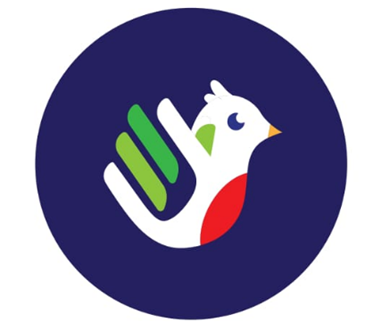
\includegraphics[width=0.4\linewidth]{figuras/logo4.png}
    \caption{Logo con colores}
    \label{fig:enter-label}
\end{figure}

Finalmente, se logró el diseño definitivo: un logo colorido y moderno que refleja la cultura de Guatemala a través del símbolo del quetzal y representa a la comunidad sorda con la imagen de una mano utilizando LENSEGUA. Este logo combina simplicidad, modernidad y simbolismo cultural, proporcionando una representación atractiva y efectiva para la aplicación. 


\begin{figure} [H]
    \centering
    
\includegraphics[width=0.4\linewidth]{figuras/logo_final.png}
    \caption{Logo Señas Chapinas}
    \label{fig:enter-label}
\end{figure}



% -----------------------------------------------------------------------------------------

\subsection{Paleta de Colores}


Los colores seleccionados para el logo son los siguientes:


\begin{itemize}
    
    \item \textbf{Verde Quetzal (\#00973A):} Este color representa al quetzal y simboliza vida y esperanza. 
       
    \item \textbf{Rojo (\#E20613):}  Su uso en la app es para indicar errores o acciones importantes, facilitando al usuario identificar problemas o acciones críticas dentro de la aplicación.

    \item \textbf{Verde Lima (\#93C01F):} Se utiliza para dar mas detalle al quetzal y para el título de la aplicación porque tiene mayor contraste con el azul del fondo. 
    
    \item \textbf{Amarillo (\#FFDD00):}) Usado para destacar el pico del quetzal en el logo, este amarillo no solo contrasta eficazmente con los verdes, sino que también simboliza felicidad y acción. 

    \item \textbf{Azul (\#29235C):}) Aunque el azul tradicional de la bandera de Guatemala es más claro, se ha seleccionado un tono azul oscuro para conferir profundidad y seriedad al logo
    
\end{itemize}

\begin{figure} [H]
    \centering
    \includegraphics[width=0.25\linewidth]{figuras/paleta_colores_logo.png}
    \caption{Paleta de colores logo}
    \label{fig:enter-label}
\end{figure}


En base a estos colores, también se seleccionaron los colores pera la aplicación, buscando no solo impacto visual, sino que también  fortalecer la conexión con la identidad cultural guatemalteca.

\begin{itemize}
    \item \textbf{Azul (\#29235C):} Se utiliza principalmente como color para texto de la aplicación. Ofrece legibilidad y una sensación de seguridad y confianza.  
    
    \item \textbf{Verde Quetzal (\#00973A):} Se usa para botones y títulos, aportando vitalidad y energía a la interfaz. 
       
    \item \textbf{Rojo (\#E20613):} Se utuliza para indicar errores o acciones importantes, facilitando al usuario identificar problemas o acciones críticas dentro de la aplicación.

    \item \textbf{Blanco Crema (\#F5F5F5):} Se utiliza como fondo para la aplicación. En lugar del blanco puro, este tono crema proporciona una suavidad que puede ser menos agresiva a la vista. 
    
    \item \textbf{Gris Carbón (\#323232):} Se utiliza principalmente como fondo de pantallas de temporales. Es un color neutro elegido específicamente para minimizar las distracciones y evitar que los usuarios permanezcan en estas pantallas transitorias por más tiempo del necesario, a diferencia del uso de los colores azul y blanco en otras secciones de la aplicación, que buscan captar y mantener la atención del usuario.

\begin{figure} [H]
    \centering
    \includegraphics[width=0.6\linewidth]{figuras/paleta_colores.png}
    \caption{Paleta de colores aplicación}
    \label{fig:enter-label}
\end{figure}

    
    
\end{itemize}

En base a la paleta de colores del logo, se obtienen colores pasteltes utilizados para el queztal de perfil del usuario y las opciones del reto diario:

\begin{itemize}

    \item Aqua Pastel (\#37B7C3)
    \item Azul Pastel (\#83B4FF)
    \item Verde Pastel (\#8DC249)
    \item Amarillo Pastel (\#FCB424)

\end{itemize}

\begin{figure} [H]
    \centering
    \includegraphics[width=0.5\linewidth]{figuras/paleta_colores_quetzal.png}
    \caption{Paleta Colores Perfil}
    \label{fig:enter-label}
\end{figure}

Asimismo también se comprueban contrastes de los colores seleccionados:

\begin{itemize}

    \item \textbf{Azul y Blanco:} Los colores azul y blanco seleccionados presentan un contraste óptimo, lo cual justifica su uso como fondo y texto principales en la aplicación. 

    \begin{figure} [H]
        \centering
        \includegraphics[width=0.6\linewidth]{figuras/contraste_azul_blanco.png}
        \caption{Contraste Blanco y Azul}
        \label{fig:enter-label}
    \end{figure}


    \begin{figure} [H]
        \centering
        \includegraphics[width=0.6\linewidth]{figuras/contraste_blanco_azul.png}
        \caption{Contraste Azul y Blanco}
        \label{fig:enter-label}
    \end{figure}

  
    \item \textbf{Contraste gris y blanco:} Los colores gris y blanco seleccionados ofrecen un contraste adecuado, lo cual los hace idóneos para su uso en las pantallas temporales. 

    \begin{figure} [H]
        \centering
        \includegraphics[width=0.6\linewidth]{figuras/contraste_gris_blanco.png}
        \caption{Contraste gris y blanco}
        \label{fig:enter-label}
    \end{figure}
    
    
    \item \textbf{Constraste blanco y rojo:}  Aunque el contraste entre blanco y rojo no es tan alto como en otros casos, aún cumple con los requisitos mínimos recomendados. Este se utiliza exclusivamente en situaciones necesarias para alertar al usuario sobre una acción crítica.

    \begin{figure} [H]
        \centering
        \includegraphics[width=0.6\linewidth]{figuras/contraste_blanco_rojo.png}
        \caption{Contraste blanco y rojo}
        \label{fig:enter-label}
    \end{figure}
    
    \item \textbf{Contraste verde quetzal y azul:} El contraste entre el verde quetzal es ligeramente inferior al nivel recomendado. Por esta razón, se empleará únicamente para elementos destacados como títulos grandes, botones y el logo, donde la legibilidad sigue siendo efectiva a pesar del menor contraste. 
   
    \begin{figure} [H]
        \centering
        \includegraphics[width=0.6\linewidth]{figuras/contraste_azul_verde.png}
        \caption{Constraste verde quetzal y azul}
        \label{fig:enter-label}
    \end{figure}

    \item \textbf{Contraste verde claro y azul:} El contraste entre el verde claro y el azul cumple con las normas recomendadas, razón por la cual se ha seleccionado para el título de la aplicación
    
    \begin{figure} [H]
        \centering
        \includegraphics[width=0.6\linewidth]{figuras/contraste_verde_claro_azul.png}
        \caption{Constraste verde claro y azul}
        \label{fig:enter-label}
    \end{figure}
        

\end{itemize}


% -----------------------------------------------------------------------------------------

\subsection{Tipografía}

La tipografía recomendada por la diseñadora gráfica para el logo de "Señas Chapinas" fue Adonide Bold. Esta elección se justifica por su claridad y modernidad, cualidades que reflejan la simplicidad y accesibilidad que la aplicación busca transmitir. Adonide Bold es una fuente sans-serif que ofrece un aspecto limpio y profesional, ideal para destacar en logotipos y cabeceras por su legibilidad y presencia  \cite{GraphiqueSF}.

En base a esa tipografía y al contexto de la aplicación, se decide utilizar Nunito para el contenido de la app. Nunito, también una sans-serif disponible gratuitamente en Google Fonts, es conocida por sus curvas suaves y su legibilidad en interfaces digitales, lo que la hace ideal para textos largos y elementos de interfaz de usuario en aplicaciones móviles. Su diseño amigable y accesible complementa perfectamente la estética introducida por Adonide Bold en el logo, asegurando coherencia visual y facilitando la experiencia del usuario al navegar por la aplicación. Esta elección refuerza el objetivo de la app de ser accesible y fácil de usar, elementos cruciales para una herramienta destinada a mejorar la comunicación en la comunidad sorda \cite{Design2024}.

\begin{figure} [H]
    \centering
    \includegraphics[width=0.75\linewidth]{figuras/tipografia.png}
    \caption{Tipografía Nunito}
    \label{fig:enter-label}
\end{figure}

% -----------------------------------------------------------------------------------------

\subsection{Prototipos}

Al concluir la fase de diseño UX/UI, se han definido claramente las necesidades de los usuarios, así como los flujos principales de la aplicación. Durante este proceso, también se seleccionaron cuidadosamente los colores y la tipografía que mejor se adaptan a la experiencia del usuario, garantizando así coherencia visual y funcionalidad. Con estos elementos bien establecidos, el siguiente paso ha sido la creación de prototipos detallados en Figma. Este enfoque permite simular la interacción del usuario con la aplicación, 


\begin{itemize}

    \item \textbf{Prototipo de Bajo Nivel:} Este primer prototipo tiene como objetivo demostrar la funcionalidad general de la aplicación sin enfocarse en el diseño de colores, presentando una estructura básica. Para ver el diseño con más detalles consultar: \href{https://www.figma.com/design/d7NOw36r1mUY7qDBIveJ2K/Se%C3%B1as-Chapinas?node-id=45-820&node-type=SECTION&t=luJsnsyUNaEJGP24-0}{Figma}.


    \begin{itemize}
        \item \textbf{Barra de Navegación:} Contiene las opciones de "Video", "Traductor", "Diccionario" y "Perfil". La opción seleccionada se destaca visualmente sobre las demás.
        
        \item \textbf{Pantalla de Inicio:} Ofrece la función principal de grabar video. Al presionar el botón correspondiente, el video comienza a grabarse.
        
        \item \textbf{Pantalla de Video:} Muestra el video grabado junto con opciones para reportar errores, agregar a favoritos, compartir, repetir, utilizar el altavoz y cerrar. Las traducciones en español y LENSEGUA se muestran en la parte inferior.
        
        \item \textbf{Reporte de Traducción:} Un modal que permite al usuario reportar errores en la traducción. Antes de continuar, se solicita revisar el diccionario. Luego, el usuario puede proceder con el reporte.
        
        \item \textbf{Traductor:} Al ingresar, se presenta un área para escribir o pegar texto en LENSEGUA. El botón de traducción está deshabilitado hasta que el usuario ingrese el texto. Una vez ingresado, el botón se habilita, y al presionarlo, se muestra la traducción al español junto con las opciones de copiar, escuchar con el altavoz, agregar a favoritos o realizar una nueva traducción.
        
        \item \textbf{Diccionario:} Muestra tarjetas redondeadas que representan las palabras disponibles. Las tarjetas se pueden agregar a favoritos. En la parte superior, se incluye una barra de búsqueda y la opción de seleccionar por categorías. Además, cuenta con una barra de desplazamiento para navegar entre las tarjetas ordenadas alfabéticamente.
        
        \item \textbf{Perfil del Usuario:} Muestra una imagen de perfil, el nombre del usuario y un contador de días consecutivos de desafíos completados. También incluye un ícono de configuración en la parte superior para acceder a ajustes. La pantalla presenta una barra de pestañas que permite alternar entre los videos favoritos y las traducciones favoritas.
        
        \item \textbf{Configuraciones:} Ofrece opciones para cambiar la contraseña, cerrar sesión, eliminar la cuenta y acceder a información sobre la aplicación. También permite activar o desactivar los retos diarios, ver un tutorial y consultar la versión actual de la app.
        
        \item \textbf{Retos Diarios:} Presenta cuatro imágenes como opciones de respuesta para una palabra en LENSEGUA. El usuario puede elegir una respuesta, o bien, cerrar u omitir el reto. Las opciones se presentan en un diálogo interactivo.
    \end{itemize}
    
    \begin{figure} [H]
        \centering
        \includegraphics[width=1\linewidth]{figuras/Prototipo1.png}
        \caption{Primer Prototipo}
        \label{fig:enter-label}
    \end{figure}

    
    \item \textbf{Segundo Prototipo} 

    \begin{figure} [H]
        \centering
        \includegraphics[width=1\linewidth]{figuras/segundo_prototipo.png}
        \caption{Segundo Prototipo}
        \label{fig:enter-label}
    \end{figure}


    \item \textbf{Tercer Prototipo} 

    \begin{figure} [H]
        \centering
        \includegraphics[width=1\linewidth]{figuras/segundo_prototipo.png}
        \caption{Tercer prototipo}
        \label{fig:enter-label}
    \end{figure}

\end{itemize}

% ===========================================================================================

\section{DESARROLLO MÓVIL}

% ===========================================================================================

\section{PRUEBAS CON USUARIOS FINALES}